%------------------------------------------------------------------
% !TEX program = xelatex
% !BIB program = biber
%------------------------------------------------------------------
%&preformat-disser
%\RequirePackage[l2tabu,orthodox]{nag} % Раскомментировав, можно в логе получать рекомендации относительно правильного использования пакетов и предупреждения об устаревших и нерекомендуемых пакетах
% Формат А4, 14pt (ГОСТ Р 7.0.11-2011, 5.3.6)
\documentclass[a4paper,14pt,oneside,openany]{memoir}

%%% Проверка используемого TeX-движка %%%
\RequirePackage{ifxetex, ifluatex}
\newif\ifxetexorluatex   % определяем новый условный оператор (http://tex.stackexchange.com/a/47579)
\ifxetex
    \xetexorluatextrue
\else
    \ifluatex
        \xetexorluatextrue
    \else
        \xetexorluatexfalse
    \fi
\fi

\newif\ifsynopsis           % Условие, проверяющее, что документ --- автореферат
\RequirePackage{etoolbox}[2015/08/02]               % Для продвинутой проверки разных условий

%%% Поля и разметка страницы %%%
\usepackage{pdflscape}                              % Для включения альбомных страниц
\usepackage{geometry}                               % Для последующего задания полей

%%% Математические пакеты %%%
\usepackage{amsthm,amsmath,amscd,amsfonts,amssymb}  % Математические дополнения от AMS
\usepackage{mathtools}                              % Добавляет окружение multlined
\usepackage{unicode-math}
\usepackage{amstext}                               % Русские символы в формулах

%%%% Установки для размера шрифта 14 pt %%%%
%% Формирование переменных и констант для сравнения (один раз для всех подключаемых файлов)%%
%% должно располагаться до вызова пакета fontspec или polyglossia, потому что они сбивают его работу
\newlength{\curtextsize}
\newlength{\bigtextsize}
\setlength{\bigtextsize}{13.9pt}

\makeatletter
%\show\f@size                                       % неплохо для отслеживания, но вызывает стопорение процесса, если документ компилируется без команды  -interaction=nonstopmode
\setlength{\curtextsize}{\f@size pt}
\makeatother

%%% Кодировки и шрифты %%%
\usepackage{polyglossia}[2014/05/21]            % Поддержка многоязычности (fontspec подгружается автоматически)

%%% Оформление абзацев %%%
\usepackage{indentfirst}                            % Красная строка

%%% Цвета %%%
\usepackage[dvipsnames, table, hyperref, cmyk]{xcolor} % Совместимо с tikz. Конвертация всех цветов в cmyk заложена как удовлетворение возможного требования типографий. Возможно конвертирование и в rgb.

%%% Таблицы %%%
\usepackage{longtable,ltcaption}                    % Длинные таблицы
\usepackage{multirow,makecell}                      % Улучшенное форматирование таблиц

%%% Общее форматирование
\usepackage{soulutf8}                               % Поддержка переносоустойчивых подчёркиваний и зачёркиваний
\usepackage{icomma}                                 % Запятая в десятичных дробях
\usepackage[hyphenation, lastparline]{impnattypo}   % Оптимизация расстановки переносов и длины последней строки абзаца

%%% Гиперссылки %%%
\usepackage{hyperref}[2012/11/06]

%%% Изображения %%%
\usepackage{graphicx}[2014/04/25]                   % Подключаем пакет работы с графикой

%%% Списки %%%
\usepackage{enumitem}

%%% Счётчики %%%
\usepackage[figure,table]{totalcount}               % Счётчик рисунков и таблиц
\usepackage{totcount}                               % Пакет создания счётчиков на основе последнего номера подсчитываемого элемента (может требовать дважды компилировать документ)
\usepackage{totpages}                               % Счётчик страниц, совместимый с hyperref (ссылается на номер последней страницы). Желательно ставить последним пакетом в преамбуле
\usepackage{pdfpages}
%%% Продвинутое управление групповыми ссылками (пока только формулами) %%%
\usepackage{cleveref}                           % cleveref корректно считывает язык из настроек polyglossia

\creflabelformat{equation}{#2#1#3}                  % Формат по умолчанию ставил круглые скобки вокруг каждого номера ссылки, теперь просто номера ссылок без какого-либо дополнительного оформления
\crefrangelabelformat{equation}{#3#1#4---#5#2#6}   % Интервалы в русском языке принято делать через тире, если иное не оговорено


%%% Цитата, не приводимая в автореферате:
% возможно, актуальна только для biblatex
%\newcommand{\citeinsynopsis}[1]{\ifsynopsis\else ~\cite{#1} \fi}
  % Пакеты общие для диссертации и автореферата
%%% Прикладные пакеты %%%
%\usepackage{calc}               % Пакет для расчётов параметров, например длины

%%% Для добавления Стр. над номерами страниц в оглавлении
%%% http://tex.stackexchange.com/a/306950
\usepackage{afterpage}

\usepackage{tikz}                   % Продвинутый пакет векторной графики
\usetikzlibrary{chains}             % Для примера tikz рисунка
\usetikzlibrary{shapes.geometric}   % Для примера tikz рисунка
\usetikzlibrary{shapes.symbols}     % Для примера tikz рисунка
\usetikzlibrary{arrows}             % Для примера tikz рисунка

\usepackage[explicit]{titlesec}   %
\usepackage{tocvsec2}               %Подробности оглавления
 \usepackage[normalem]{ulem}
 \useunder{\uline}{\ul}{}
%\usepackage{titlesec}%
%\usepackage{caption}
%\usepackage{subcaption}
%\usepackage{subfig}
         % Пакеты для диссертации
\usepackage{tabu, tabulary}  %таблицы с автоматически подбирающейся шириной столбцов
\usepackage{fr-longtable}    %ради \endlasthead

% Листинги с исходным кодом программ
\usepackage{fancyvrb}
\usepackage{listings}
\lccode`\~=0\relax %Без этого хака из-за особенностей пакета listings перестают работать конструкции с \MakeLowercase и т. п. в (xe|lua)latex

% Русская традиция начертания греческих букв
\usepackage{upgreek} % прямые греческие ради русской традиции

% Микротипографика
%    \usepackage[final]{microtype}[2016/05/14] % улучшает представление букв и слов в строках, может помочь при наличии отдельно висящих слов

        % Пакеты для специфических пользовательских задач

%%%%%%%%%%%%%%%%%%%%%%%%%%%%%%%%%%%%%%%%%%%%%%%%%%%%%%
%%%% Файл упрощённых настроек шаблона диссертации %%%%
%%%%%%%%%%%%%%%%%%%%%%%%%%%%%%%%%%%%%%%%%%%%%%%%%%%%%%

%%% Инициализирование переменных, не трогать!  %%%
\newcounter{intvl}
\newcounter{otstup}
\newcounter{contnumeq}
\newcounter{contnumfig}
\newcounter{contnumtab}
\newcounter{pgnum}
\newcounter{chapstyle}
\newcounter{headingdelim}
\newcounter{headingalign}
\newcounter{headingsize}
\newcounter{tabcap}
\newcounter{tablaba}
\newcounter{tabtita}
\newcounter{usefootcite}
%% Мои указатели
%%%%%%%%%%%%%%%%%%%%%%%%%%%%%%%%%%%%%%%%%%%%%%%%%%

%%% Область упрощённого управления оформлением %%%

%% Интервал между заголовками и между заголовком и текстом
% Заголовки отделяют от текста сверху и снизу тремя интервалами (ГОСТ Р 7.0.11-2011, 5.3.5)
\setcounter{intvl}{2}               % Коэффициент кратности к размеру шрифта

%% Отступы у заголовков в тексте
\setcounter{otstup}{1}              % 0 --- без отступа; 1 --- абзацный отступ

%% Нумерация формул, таблиц и рисунков
\setcounter{contnumeq}{0}           % Нумерация формул: 0 --- пораздельно (во введении подряд, без номера раздела); 1 --- сквозная нумерация по всей диссертации
\setcounter{contnumfig}{0}          % Нумерация рисунков: 0 --- пораздельно (во введении подряд, без номера раздела); 1 --- сквозная нумерация по всей диссертации
\setcounter{contnumtab}{0}          % Нумерация таблиц: 0 --- пораздельно (во введении подряд, без номера раздела); 1 --- сквозная нумерация по всей диссертации

%% Оглавление
\setcounter{pgnum}{0}               % 0 --- номера страниц никак не обозначены; 1 --- Стр. над номерами страниц (дважды компилировать после изменения)
\settocdepth{section}            % до какого уровня подразделов выносить в оглавление
\setsecnumdepth{none}         % до какого уровня нумеровать подразделы


%% Текст и форматирование заголовков
\setcounter{chapstyle}{0}           % 0 --- разделы только под номером; 1 --- разделы с названием "Глава" перед номером
\setcounter{headingdelim}{0}        % 0 --- номер отделен пропуском в 1em или \quad; 1 --- номера разделов и приложений отделены точкой с пробелом, подразделы пропуском без точки; 2 --- номера разделов, подразделов и приложений отделены точкой с пробелом.

%% Выравнивание заголовков в тексте
\setcounter{headingalign}{0}        % 0 --- по центру; 1 --- по левому краю

%% Размеры заголовков в тексте
\setcounter{headingsize}{0}         % 0 --- по ГОСТ, все всегда 14 пт; 1 --- пропорционально изменяющийся размер в зависимости от базового шрифта

%% Подпись таблиц
\setcounter{tabcap}{0}              % 0 --- по ГОСТ, номер таблицы и название разделены тире, выровнены по левому краю, при необходимости на нескольких строках; 1 --- подпись таблицы не по ГОСТ, на двух и более строках, дальнейшие настройки:
%Выравнивание первой строки, с подписью и номером
\setcounter{tablaba}{0}             % 0 --- по левому краю; 1 --- по центру; 2 --- по правому краю
%Выравнивание строк с самим названием таблицы
\setcounter{tabtita}{0}             % 0 --- по левому краю; 1 --- по центру; 2 --- по правому краю
%Разделитель записи «Таблица #» и названия таблицы
\newcommand{\tablabelsep}{\ }

%% Подпись рисунков
%Разделитель записи «Рисунок #» и названия рисунка
\newcommand{\figlabelsep}{~\textemdash\ } % (ГОСТ 2.105, 4.3.1) % "--- здесь не работает

%%% Цвета гиперссылок %%%
% Latex color definitions: http://latexcolor.com/
\definecolor{linkcolor}{rgb}{0.9,0,0}
\definecolor{citecolor}{rgb}{0,0.6,0}
\definecolor{urlcolor}{rgb}{0,0,1}
%\definecolor{linkcolor}{rgb}{0,0,0} %black
%\definecolor{citecolor}{rgb}{0,0,0} %black
%\definecolor{urlcolor}{rgb}{0,0,0} %black
               % Упрощённые настройки шаблона

%%% Переопределение именований, чтобы можно было и в преамбуле использовать %%%
\renewcommand{\chaptername}{Практична робота}
\renewcommand{\appendixname}{Додаток} % (ГОСТ Р 7.0.11-2011, 5.7)
       % Переопределение именований, чтобы можно было и в преамбуле использовать
% Новые переменные, которые могут использоваться во всём проекте
% ГОСТ 7.0.11-2011
% 9.2 Оформление текста автореферата диссертации
% 9.2.1 Общая характеристика работы включает в себя следующие основные структурные
% элементы:
% актуальность темы исследования;
\newcommand{\actualityTXT}{Актуальность темы.}
% степень ее разработанности;
\newcommand{\progressTXT}{Степень разработанности темы.}
% цели и задачи;
\newcommand{\aimTXT}{Целью}
\newcommand{\tasksTXT}{задачи}
% научную новизну;
\newcommand{\noveltyTXT}{Научная новизна:}
% теоретическую и практическую значимость работы;
%\newcommand{\influenceTXT}{Теоретическая и практическая значимость}
% или чаще используют просто
\newcommand{\influenceTXT}{Практическая значимость}
% методологию и методы исследования;
\newcommand{\methodsTXT}{Mетодология и методы исследования.}
% положения, выносимые на защиту;
\newcommand{\defpositionsTXT}{Основные положения, выносимые на~защиту:}
% степень достоверности и апробацию результатов.
\newcommand{\reliabilityTXT}{Достоверность}
\newcommand{\probationTXT}{Апробация работы.}

\newcommand{\contributionTXT}{Личный вклад.}
\newcommand{\publicationsTXT}{Публикации.}


\newcommand{\authorbibtitle}{Публикации автора по теме диссертации}
\newcommand{\vakbibtitle}{В изданиях из списка ВАК РФ}
\newcommand{\notvakbibtitle}{В прочих изданиях}
\newcommand{\confbibtitle}{В сборниках трудов конференций}
\newcommand{\fullbibtitle}{Список використаних джерел} % (ГОСТ Р 7.0.11-2011, 4)
\newcommand{\conname}{Fernando De Luca}
  % Новые переменные, которые могут использоваться во всём проекте

%%% Основные сведения %%%
\newcommand{\thesisAuthorLastName}{\todo{Фамилия}}
\newcommand{\thesisAuthorOtherNames}{\todo{Имя Отчество}}
\newcommand{\thesisAuthorInitials}{\todo{И.\,О.}}
\newcommand{\thesisAuthor}             % Диссертация, ФИО автора
{%
    \texorpdfstring{% \texorpdfstring takes two arguments and uses the first for (La)TeX and the second for pdf
        \thesisAuthorLastName~\thesisAuthorOtherNames% так будет отображаться на титульном листе или в тексте, где будет использоваться переменная
    }{%
        \thesisAuthorLastName, \thesisAuthorOtherNames% эта запись для свойств pdf-файла. В таком виде, если pdf будет обработан программами для сбора библиографических сведений, будет правильно представлена фамилия.
    }
}
\newcommand{\thesisAuthorShort}        % Диссертация, ФИО автора инициалами
{\thesisAuthorInitials~\thesisAuthorLastName}
%\newcommand{\thesisUdk}                % Диссертация, УДК
%{\todo{xxx.xxx}}
\newcommand{\thesisTitle}              % Диссертация, название
{\todo{Название диссертационной работы}}
\newcommand{\thesisSpecialtyNumber}    % Диссертация, специальность, номер
{\todo{XX.XX.XX}}
\newcommand{\thesisSpecialtyTitle}     % Диссертация, специальность, название
{\todo{Название специальности}}
\newcommand{\thesisDegree}             % Диссертация, ученая степень
{\todo{кандидата физико-математических наук}}
\newcommand{\thesisDegreeShort}        % Диссертация, ученая степень, краткая запись
{\todo{канд. физ.-мат. наук}}
\newcommand{\thesisCity}               % Диссертация, город написания диссертации
{\todo{Город}}
\newcommand{\thesisYear}               % Диссертация, год написания диссертации
{\todo{20XX}}
\newcommand{\thesisOrganization}       % Диссертация, организация
{\todo{Название учреждения, в~котором выполнялась данная диссертационная работа}}
\newcommand{\thesisOrganizationShort}  % Диссертация, краткое название организации для доклада
{\todo{НазУчДисРаб}}

\newcommand{\thesisInOrganization}     % Диссертация, организация в предложном падеже: Работа выполнена в ...
{\todo{учреждении, в~котором выполнялась данная диссертационная работа}}

\newcommand{\supervisorFio}            % Научный руководитель, ФИО
{\todo{Фамилия Имя Отчество}}
\newcommand{\supervisorRegalia}        % Научный руководитель, регалии
{\todo{уч. степень, уч. звание}}
\newcommand{\supervisorFioShort}       % Научный руководитель, ФИО
{\todo{И.\,О.~Фамилия}}
\newcommand{\supervisorRegaliaShort}   % Научный руководитель, регалии
{\todo{уч.~ст.,~уч.~зв.}}


\newcommand{\opponentOneFio}           % Оппонент 1, ФИО
{\todo{Фамилия Имя Отчество}}
\newcommand{\opponentOneRegalia}       % Оппонент 1, регалии
{\todo{доктор физико-математических наук, профессор}}
\newcommand{\opponentOneJobPlace}      % Оппонент 1, место работы
{\todo{Не очень длинное название для места работы}}
\newcommand{\opponentOneJobPost}       % Оппонент 1, должность
{\todo{старший научный сотрудник}}

\newcommand{\opponentTwoFio}           % Оппонент 2, ФИО
{\todo{Фамилия Имя Отчество}}
\newcommand{\opponentTwoRegalia}       % Оппонент 2, регалии
{\todo{кандидат физико-математических наук}}
\newcommand{\opponentTwoJobPlace}      % Оппонент 2, место работы
{\todo{Основное место работы c длинным длинным длинным длинным названием}}
\newcommand{\opponentTwoJobPost}       % Оппонент 2, должность
{\todo{старший научный сотрудник}}

\newcommand{\leadingOrganizationTitle} % Ведущая организация, дополнительные строки
{\todo{Федеральное государственное бюджетное образовательное учреждение высшего профессионального образования с~длинным длинным длинным длинным названием}}

\newcommand{\defenseDate}              % Защита, дата
{\todo{DD mmmmmmmm YYYY~г.~в~XX часов}}
\newcommand{\defenseCouncilNumber}     % Защита, номер диссертационного совета
{\todo{Д\,123.456.78}}
\newcommand{\defenseCouncilTitle}      % Защита, учреждение диссертационного совета
{\todo{Название учреждения}}
\newcommand{\defenseCouncilAddress}    % Защита, адрес учреждение диссертационного совета
{\todo{Адрес}}
\newcommand{\defenseCouncilPhone}      % Телефон для справок
{\todo{+7~(0000)~00-00-00}}

\newcommand{\defenseSecretaryFio}      % Секретарь диссертационного совета, ФИО
{\todo{Фамилия Имя Отчество}}
\newcommand{\defenseSecretaryRegalia}  % Секретарь диссертационного совета, регалии
{\todo{д-р~физ.-мат. наук}}            % Для сокращений есть ГОСТы, например: ГОСТ Р 7.0.12-2011 + http://base.garant.ru/179724/#block_30000

\newcommand{\synopsisLibrary}          % Автореферат, название библиотеки
{\todo{Название библиотеки}}
\newcommand{\synopsisDate}             % Автореферат, дата рассылки
{\todo{DD mmmmmmmm YYYY года}}

% To avoid conflict with beamer class use \providecommand
\providecommand{\keywords}%            % Ключевые слова для метаданных PDF диссертации и автореферата
{}
      % Основные сведения
%%% Шаблон %%%
\DeclareRobustCommand{\todo}{\textcolor{red}}       % решаем проблему превращения названия цвета в результате \MakeUppercase, http://tex.stackexchange.com/a/187930/79756 , \DeclareRobustCommand protects \todo from expanding inside \MakeUppercase
\AtBeginDocument{%
    \setlength{\parindent}{2.5em}                   % Абзацный отступ. Должен быть одинаковым по всему тексту и равен пяти знакам (ГОСТ Р 7.0.11-2011, 5.3.7).
}

%%% Кодировки и шрифты %%%
\setmainlanguage{ukrainian}  % Язык по-умолчанию русский с поддержкой приятных команд пакета babel
\setotherlanguages{russian,english}                       % Дополнительный язык = английский (в американской вариации по-умолчанию)
\setmonofont{Courier New}                        % моноширинный шрифт
\newfontfamily\cyrillicfonttt{Courier New}       % моноширинный шрифт для кириллицы
\defaultfontfeatures{Ligatures=TeX}              % стандартные лигатуры TeX, замены нескольких дефисов на тире и т. п. Настройки моноширинного шрифта должны идти до этой строки, чтобы при врезках кода программ в коде не применялись лигатуры и замены дефисов
\setmainfont{Times New Roman}                    % Шрифт с засечками
\newfontfamily\cyrillicfont{Times New Roman}     % Шрифт с засечками для кириллицы
\setsansfont{Arial}                              % Шрифт без засечек
\newfontfamily\cyrillicfontsf{Arial}             % Шрифт без засечек для кириллицы


%%% Подписи %%%
\setlength{\abovecaptionskip}{0pt}   % Отбивка над подписью
\setlength{\belowcaptionskip}{0pt}   % Отбивка под подписью
\captionwidth{\linewidth}
\normalcaptionwidth

%%% Таблицы %%%
\ifnumequal{\value{tabcap}}{0}{%
    \newcommand{\tabcapalign}{\raggedright \hspace{2.5em}}  % по левому краю страницы или аналога parbox
    \renewcommand{\tablabelsep}{~\textemdash\ } % тире как разделитель идентификатора с номером от наименования
    \newcommand{\tabtitalign}{}
}{%
    \ifnumequal{\value{tablaba}}{0}{%
        \newcommand{\tabcapalign}{\raggedright}  % по левому краю страницы или аналога parbox
    }{}

    \ifnumequal{\value{tablaba}}{1}{%
        \newcommand{\tabcapalign}{\centering}    % по центру страницы или аналога parbox
    }{}

    \ifnumequal{\value{tablaba}}{2}{%
        \newcommand{\tabcapalign}{\raggedleft}   % по правому краю страницы или аналога parbox
    }{}

    \ifnumequal{\value{tabtita}}{0}{%
        \newcommand{\tabtitalign}{\par\raggedright}  % по левому краю страницы или аналога parbox
    }{}

    \ifnumequal{\value{tabtita}}{1}{%
        \newcommand{\tabtitalign}{\par\centering}    % по центру страницы или аналога parbox
    }{}

    \ifnumequal{\value{tabtita}}{2}{%
        \newcommand{\tabtitalign}{\par\raggedleft}   % по правому краю страницы или аналога parbox
    }{}
}

\precaption{\tabcapalign} % всегда идет перед подписью или \legend
\captionnamefont{\normalfont\normalsize} % Шрифт надписи «Таблица #»; также определяет шрифт у \legend
\captiondelim{\tablabelsep} % разделитель идентификатора с номером от наименования
\captionstyle[\tabtitalign]{\tabtitalign}
\captiontitlefont{\normalfont\normalsize} % Шрифт с текстом подписи


%%% Рисунки %%%
\setfloatadjustment{figure}{%
    \setlength{\abovecaptionskip}{0pt}   % Отбивка над подписью
    \setlength{\belowcaptionskip}{0pt}   % Отбивка под подписью
    \precaption{} % всегда идет перед подписью или \legend
    \captionnamefont{\normalfont\normalsize} % Шрифт надписи «Рисунок #»; также определяет шрифт у \legend
    \captiondelim{\figlabelsep} % разделитель идентификатора с номером от наименования
    \captionstyle[\centering]{\centering} % Центрирование подписей, заданных командой \caption и \legend
    \captiontitlefont{\normalfont\normalsize} % Шрифт с текстом подписи
    \postcaption{} % всегда идет после подписи или \legend, и с новой строки
}

%%% Подписи подрисунков %%%
\newsubfloat{figure} % Включает возможность использовать подрисунки у окружений figure
\renewcommand{\thesubfigure}{\asbuk{subfigure}}           % Буквенные номера подрисунков
\subcaptionsize{\normalsize} % Шрифт подписи названий подрисунков (не отличается от основного)
\subcaptionlabelfont{\normalfont}
\subcaptionfont{\!\!) \normalfont} % Вот так тут добавили скобку после буквы.
\subcaptionstyle{\centering}
%\subcaptionsize{\fontsize{12pt}{13pt}\selectfont} % объявляем шрифт 12pt для использования в подписях, тут же надо интерлиньяж объявлять, если не наследуется

%%% Настройки гиперссылок %%%
\ifluatex
    \hypersetup{
        unicode,                % Unicode encoded PDF strings
    }
\fi

\hypersetup{
    linktocpage=true,           % ссылки с номера страницы в оглавлении, списке таблиц и списке рисунков
%    linktoc=all,                % both the section and page part are links
%    pdfpagelabels=false,        % set PDF page labels (true|false)
    plainpages=false,           % Forces page anchors to be named by the Arabic form  of the page number, rather than the formatted form
    colorlinks,                 % ссылки отображаются раскрашенным текстом, а не раскрашенным прямоугольником, вокруг текста
    linkcolor={linkcolor},      % цвет ссылок типа ref, eqref и подобных
    citecolor={citecolor},      % цвет ссылок-цитат
    urlcolor={urlcolor},        % цвет гиперссылок
%    hidelinks,                  % Hide links (removing color and border)
    pdftitle={\thesisTitle},    % Заголовок
    pdfauthor={\thesisAuthor},  % Автор
    pdfsubject={\thesisSpecialtyNumber\ \thesisSpecialtyTitle},      % Тема
%    pdfcreator={Создатель},     % Создатель, Приложение
%    pdfproducer={Производитель},% Производитель, Производитель PDF
    pdfkeywords={\keywords},    % Ключевые слова
    pdflang={ru},
}

%%% Списки %%%
% Используем короткое тире (endash) для ненумерованных списков (ГОСТ 2.105-95, пункт 4.1.7, требует дефиса, но так лучше смотрится)
\renewcommand{\labelitemi}{\normalfont\bfseries{--}}

% Перечисление строчными буквами латинского алфавита (ГОСТ 2.105-95, 4.1.7)
%\renewcommand{\theenumi}{\alph{enumi}}
%\renewcommand{\labelenumi}{\theenumi)}

% Перечисление строчными буквами русского алфавита (ГОСТ 2.105-95, 4.1.7)
\makeatletter
\AddEnumerateCounter{\asbuk}{\russian@alph}{щ}      % Управляем списками/перечислениями через пакет enumitem, а он 'не знает' про asbuk, потому 'учим' его
\makeatother
%\renewcommand{\theenumi}{\asbuk{enumi}} %первый уровень нумерации
%\renewcommand{\labelenumi}{\theenumi)} %первый уровень нумерации
\renewcommand{\theenumii}{\asbuk{enumii}} %второй уровень нумерации
\renewcommand{\labelenumii}{\theenumii)} %второй уровень нумерации
\renewcommand{\theenumiii}{\arabic{enumiii}} %третий уровень нумерации
\renewcommand{\labelenumiii}{\theenumiii)} %третий уровень нумерации

\setlist{nosep,%                                    % Единый стиль для всех списков (пакет enumitem), без дополнительных интервалов.
    labelindent=\parindent,leftmargin=*%            % Каждый пункт, подпункт и перечисление записывают с абзацного отступа (ГОСТ 2.105-95, 4.1.8)
}
    % Стили общие для диссертации и автореферата

%%% Изображения %%%
\graphicspath{{images/}}         % Пути к изображениям

%%% Макет страницы %%%
% Выставляем значения полей (ГОСТ 7.0.11-2011, 5.3.7)
\geometry{a4paper,top=2cm,bottom=2cm,left=2.5cm,right=1cm,nofoot,nomarginpar} %,showframe
\setlength{\topskip}{0pt}   %размер дополнительного верхнего поля
\setlength{\footskip}{12.3pt} % снимет warning, согласно https://tex.stackexchange.com/a/334346

%%% Интервалы %%%
%% По ГОСТ Р 7.0.11-2011, пункту 5.3.6 требуется полуторный интервал
%% Реализация средствами класса (на основе setspace) ближе к типографской классике.
%% И правит сразу и в таблицах (если со звёздочкой)
%\DoubleSpacing*     % Двойной интервал
\OnehalfSpacing*    % Полуторный интервал
%\setSpacing{1.42}   % Полуторный интервал, подобный Ворду (возможно, стоит включать вместе с предыдущей строкой)

%%% Выравнивание и переносы %%%
%% http://tex.stackexchange.com/questions/241343/what-is-the-meaning-of-fussy-sloppy-emergencystretch-tolerance-hbadness
%% http://www.latex-community.org/forum/viewtopic.php?p=70342#p70342
\tolerance 1414 %
\hbadness 1414%
\emergencystretch 1.5em % В случае проблем регулировать в первую очередь
\hfuzz 0.3pt
\vfuzz \hfuzz
%\raggedbottom
\sloppy                 % Избавляемся от переполнений
\clubpenalty=10000      % Запрещаем разрыв страницы после первой строки абзаца
\flushbottom
\widowpenalty=4991     % Запрещаем разрыв страницы после последней строки абзаца


%%% Блок управления параметрами для выравнивания заголовков в тексте %%%
\newlength{\otstuplen}
\setlength{\otstuplen}{\theotstup\parindent}
\ifnumequal{\value{headingalign}}{0}{% выравнивание заголовков в тексте
    \newcommand{\hdngalign}{\centering}                % по центру
    \newcommand{\hdngaligni}{}% по центру
    \setlength{\otstuplen}{0pt}
}{%
    \newcommand{\hdngalign}{}                 % по левому краю
    \newcommand{\hdngaligni}{\hspace{\otstuplen}}      % по левому краю
} % В обоих случаях вроде бы без переноса, как и надо (ГОСТ Р 7.0.11-2011, 5.3.5)

%%% Оглавление %%%
\renewcommand{\cftchapterdotsep}{\cftdotsep}                % отбивка точками до номера страницы начала главы/раздела

%% Переносить слова в заголовке не допускается (ГОСТ Р 7.0.11-2011, 5.3.5). Заголовки в оглавлении должны точно повторять заголовки в тексте (ГОСТ Р 7.0.11-2011, 5.2.3). Прямого указания на запрет переносов в оглавлении нет, но по той же логике невнесения искажений в смысл, лучше в оглавлении не переносить:
\setrmarg{2.55em plus1fil}                             %To have the (sectional) titles in the ToC, etc., typeset ragged right with no hyphenation
\renewcommand{\cftchapterpagefont}{\normalfont}        % нежирные номера страниц у глав в оглавлении
\renewcommand{\cftchapterleader}{\cftdotfill{\cftchapterdotsep}}% нежирные точки до номеров страниц у глав в оглавлении
%\renewcommand{\cftchapterfont}{}                       % нежирные названия глав в оглавлении

\ifnumgreater{\value{headingdelim}}{0}{%
    \renewcommand\cftchapteraftersnum{.\space}       % добавляет точку с пробелом после номера раздела в оглавлении
}{}
\ifnumgreater{\value{headingdelim}}{1}{%
    \renewcommand\cftsectionaftersnum{.\space}       % добавляет точку с пробелом после номера подраздела в оглавлении
    \renewcommand\cftsubsectionaftersnum{.\space}    % добавляет точку с пробелом после номера подподраздела в оглавлении
    \renewcommand\cftsubsubsectionaftersnum{.\space} % добавляет точку с пробелом после номера подподподраздела в оглавлении
    \AtBeginDocument{% без этого polyglossia сама всё переопределяет
        \setsecnumformat{\csname the#1\endcsname.\space}
    }
}{%
    \AtBeginDocument{% без этого polyglossia сама всё переопределяет
        \setsecnumformat{\csname the#1\endcsname\quad}
    }
}
\renewcommand*{\cftappendixname}{\appendixname\space} % Слово Приложение в оглавлении

%%% Колонтитулы %%%
% Порядковый номер страницы печатают на середине верхнего поля страницы (ГОСТ Р 7.0.11-2011, 5.3.8)
\makeevenhead{plain}{}{}{\thepage}%
 \makeoddhead{plain}{}{}{\thepage}%
\makeevenfoot{plain}{}{}{}%
\makeoddfoot{plain}{}{}{}%
\pagestyle{plain}%

%%% добавить Стр. над номерами страниц в оглавлении
%%% http://tex.stackexchange.com/a/306950
\newif\ifendTOC

\newcommand*{\tocheader}{
\ifnumequal{\value{pgnum}}{1}{%
    \ifendTOC\else\hbox to \linewidth%
      {\noindent{}~\hfill{Стр.}}\par%
      \ifnumless{\value{page}}{3}{}{%
        \vspace{0.5\onelineskip}
      }
      \afterpage{\tocheader}
    \fi%
}{}%
}%

%%% Оформление заголовков глав, разделов, подразделов %%%
%% Работа должна быть выполнена ... размером шрифта 12-14 пунктов (ГОСТ Р 7.0.11-2011, 5.3.8). То есть не должно быть надписей шрифтом более 14. Так и поставим.
%% Эти установки будут давать одинаковый результат независимо от выбора базовым шрифтом 12 пт или 14 пт
\newcommand{\basegostsectionfont}{\fontsize{14pt}{16pt}\selectfont\bfseries}

\makechapterstyle{thesisgost}{%
    \chapterstyle{default}
    \setlength{\beforechapskip}{0pt}
    \setlength{\midchapskip}{0pt}
    \setlength{\afterchapskip}{\theintvl\curtextsize}
    \renewcommand*{\chapnamefont}{\basegostsectionfont}
    \renewcommand*{\chapnumfont}{\basegostsectionfont}
    \renewcommand*{\chaptitlefont}{\basegostsectionfont}
    \renewcommand*{\chapterheadstart}{}
    \ifnumgreater{\value{headingdelim}}{0}{%
        \renewcommand*{\afterchapternum}{.\space}   % добавляет точку с пробелом после номера раздела
    }{%
        \renewcommand*{\afterchapternum}{\quad}     % добавляет \quad после номера раздела
    }
    \renewcommand*{\printchapternum}{\hdngaligni\hdngalign\chapnumfont \thechapter}
    \renewcommand*{\printchaptername}{}
    \renewcommand*{\printchapternonum}{\hdngaligni\hdngalign}
}

\makeatletter
\makechapterstyle{thesisgostchapname}{%
    \chapterstyle{thesisgost}
    \renewcommand*{\printchapternum}{\chapnumfont \thechapter}
    \renewcommand*{\printchaptername}{\hdngaligni\hdngalign\chapnamefont \@makechapterhead} %
}
\makeatother

\chapterstyle{thesisgost}

\setsecheadstyle{\basegostsectionfont\hdngalign}
\setsecindent{\otstuplen}

\setsubsecheadstyle{\basegostsectionfont\hdngalign}
\setsubsecindent{\otstuplen}

\setsubsubsecheadstyle{\basegostsectionfont\hdngalign}
\setsubsubsecindent{\otstuplen}

\sethangfrom{\noindent #1} %все заголовки подразделов центрируются с учетом номера, как block

\ifnumequal{\value{chapstyle}}{1}{%
    \chapterstyle{thesisgostchapname}
    \renewcommand*{\cftchaptername}{\chaptertitlename\space} % будет вписано слово Глава перед каждым номером раздела в оглавлении
}{}%


%%% Интервалы между заголовками
%\setbeforesecskip{\theintvl\curtextsize}% Заголовки отделяют от текста сверху и снизу тремя интервалами (ГОСТ Р 7.0.11-2011, 5.3.5).
%\setaftersecskip{\theintvl\curtextsize}
%\setbeforesubsecskip{\theintvl\curtextsize}
%\setaftersubsecskip{\theintvl\curtextsize}
%\setbeforesubsubsecskip{\theintvl\curtextsize}
%\setaftersubsubsecskip{\theintvl\curtextsize}

\setbeforesecskip{0.8ex} \setaftersecskip{0.7ex} \setbeforesubsecskip{0.8ex}
\setaftersubsecskip{0.7ex} \setbeforesubsubsecskip{0.8ex}
\setaftersubsubsecskip{0.7ex}

%%% Блок дополнительного управления размерами заголовков
\ifnumequal{\value{headingsize}}{1}{% Пропорциональные заголовки и базовый шрифт 14 пт
    \renewcommand{\basegostsectionfont}{\large\bfseries}
    \renewcommand*{\chapnamefont}{\Large\bfseries}
    \renewcommand*{\chapnumfont}{\Large\bfseries}
    \renewcommand*{\chaptitlefont}{\Large\bfseries}
}{}

%%% Счётчики %%%

%% Упрощённые настройки шаблона диссертации: нумерация формул, таблиц, рисунков
\ifnumequal{\value{contnumeq}}{1}{%
    \counterwithout{equation}{chapter} % Убираем связанность номера формулы с номером главы/раздела
}{}
\ifnumequal{\value{contnumfig}}{1}{%
    \counterwithout{figure}{chapter}   % Убираем связанность номера рисунка с номером главы/раздела
}{}
\ifnumequal{\value{contnumtab}}{1}{%
    \counterwithout{table}{chapter}    % Убираем связанность номера таблицы с номером главы/раздела
}{}


%%http://www.linux.org.ru/forum/general/6993203#comment-6994589 (используется totcount)
\makeatletter
\def\formbytotal#1#2#3#4#5{%
    \newcount\@c
    \@c\totvalue{#1}\relax
    \newcount\@last
    \newcount\@pnul
    \@last\@c\relax
    \divide\@last 10
    \@pnul\@last\relax
    \divide\@pnul 10
    \multiply\@pnul-10
    \advance\@pnul\@last
    \multiply\@last-10
    \advance\@last\@c
    \total{#1}~#2%
    \ifnum\@pnul=1#5\else%
    \ifcase\@last#5\or#3\or#4\or#4\or#4\else#5\fi
    \fi
}
\makeatother

\AtBeginDocument{
%% регистрируем счётчики в системе totcounter
    \regtotcounter{totalcount@figure}
    \regtotcounter{totalcount@table}       % Если иным способом поставить в преамбуле то ошибка в числе таблиц
    \regtotcounter{TotPages}               % Если иным способом поставить в преамбуле то ошибка в числе страниц
}

%%% Правильная нумерация приложений %%%
%% По ГОСТ 2.105, п. 4.3.8 Приложения обозначают заглавными буквами русского алфавита,
%% начиная с А, за исключением букв Ё, З, Й, О, Ч, Ь, Ы, Ъ.
%% Здесь также переделаны все нумерации русскими буквами.

\makeatletter
\def\russian@Alph#1{\ifcase#1\or
    А\or Б\or В\or Г\or Д\or Е\or Ж\or
    И\or К\or Л\or М\or Н\or
    П\or Р\or С\or Т\or У\or Ф\or Х\or
    Ц\or Ш\or Щ\or Э\or Ю\or Я\else\xpg@ill@value{#1}{russian@Alph}\fi}
\def\russian@alph#1{\ifcase#1\or
   а\or б\or в\or г\or д\or е\or ж\or
   и\or к\or л\or м\or н\or
   п\or р\or с\or т\or у\or ф\or х\or
   ц\or ш\or щ\or э\or ю\or я\else\xpg@ill@value{#1}{russian@alph}\fi}
\makeatother
           % Стили для диссертации
% для вертикального центрирования ячеек в tabulary
\def\zz{\ifx\[$\else\aftergroup\zzz\fi}
%$ \] % <-- чиним подсветку синтаксиса в некоторых редакторах
\def\zzz{\setbox0\lastbox
\dimen0\dimexpr\extrarowheight + \ht0-\dp0\relax
\setbox0\hbox{\raise-.5\dimen0\box0}%
\ht0=\dimexpr\ht0+\extrarowheight\relax
\dp0=\dimexpr\dp0+\extrarowheight\relax
\box0
}



\lstdefinelanguage{Renhanced}%
{keywords={abbreviate,abline,abs,acos,acosh,action,add1,add,%
        aggregate,alias,Alias,alist,all,anova,any,aov,aperm,append,apply,%
        approx,approxfun,apropos,Arg,args,array,arrows,as,asin,asinh,%
        atan,atan2,atanh,attach,attr,attributes,autoload,autoloader,ave,%
        axis,backsolve,barplot,basename,besselI,besselJ,besselK,besselY,%
        beta,binomial,body,box,boxplot,break,browser,bug,builtins,bxp,by,%
        c,C,call,Call,case,cat,category,cbind,ceiling,character,char,%
        charmatch,check,chol,chol2inv,choose,chull,class,close,cm,codes,%
        coef,coefficients,co,col,colnames,colors,colours,commandArgs,%
        comment,complete,complex,conflicts,Conj,contents,contour,%
        contrasts,contr,control,helmert,contrib,convolve,cooks,coords,%
        distance,coplot,cor,cos,cosh,count,fields,cov,covratio,wt,CRAN,%
        create,crossprod,cummax,cummin,cumprod,cumsum,curve,cut,cycle,D,%
        data,dataentry,date,dbeta,dbinom,dcauchy,dchisq,de,debug,%
        debugger,Defunct,default,delay,delete,deltat,demo,de,density,%
        deparse,dependencies,Deprecated,deriv,description,detach,%
        dev2bitmap,dev,cur,deviance,off,prev,,dexp,df,dfbetas,dffits,%
        dgamma,dgeom,dget,dhyper,diag,diff,digamma,dim,dimnames,dir,%
        dirname,dlnorm,dlogis,dnbinom,dnchisq,dnorm,do,dotplot,double,%
        download,dpois,dput,drop,drop1,dsignrank,dt,dummy,dump,dunif,%
        duplicated,dweibull,dwilcox,dyn,edit,eff,effects,eigen,else,%
        emacs,end,environment,env,erase,eval,equal,evalq,example,exists,%
        exit,exp,expand,expression,External,extract,extractAIC,factor,%
        fail,family,fft,file,filled,find,fitted,fivenum,fix,floor,for,%
        For,formals,format,formatC,formula,Fortran,forwardsolve,frame,%
        frequency,ftable,ftable2table,function,gamma,Gamma,gammaCody,%
        gaussian,gc,gcinfo,gctorture,get,getenv,geterrmessage,getOption,%
        getwd,gl,glm,globalenv,gnome,GNOME,graphics,gray,grep,grey,grid,%
        gsub,hasTsp,hat,heat,help,hist,home,hsv,httpclient,I,identify,if,%
        ifelse,Im,image,\%in\%,index,influence,measures,inherits,install,%
        installed,integer,interaction,interactive,Internal,intersect,%
        inverse,invisible,IQR,is,jitter,kappa,kronecker,labels,lapply,%
        layout,lbeta,lchoose,lcm,legend,length,levels,lgamma,library,%
        licence,license,lines,list,lm,load,local,locator,log,log10,log1p,%
        log2,logical,loglin,lower,lowess,ls,lsfit,lsf,ls,machine,Machine,%
        mad,mahalanobis,make,link,margin,match,Math,matlines,mat,matplot,%
        matpoints,matrix,max,mean,median,memory,menu,merge,methods,min,%
        missing,Mod,mode,model,response,mosaicplot,mtext,mvfft,na,nan,%
        names,omit,nargs,nchar,ncol,NCOL,new,next,NextMethod,nextn,%
        nlevels,nlm,noquote,NotYetImplemented,NotYetUsed,nrow,NROW,null,%
        numeric,\%o\%,objects,offset,old,on,Ops,optim,optimise,optimize,%
        options,or,order,ordered,outer,package,packages,page,pairlist,%
        pairs,palette,panel,par,parent,parse,paste,path,pbeta,pbinom,%
        pcauchy,pchisq,pentagamma,persp,pexp,pf,pgamma,pgeom,phyper,pico,%
        pictex,piechart,Platform,plnorm,plogis,plot,pmatch,pmax,pmin,%
        pnbinom,pnchisq,pnorm,points,poisson,poly,polygon,polyroot,pos,%
        postscript,power,ppoints,ppois,predict,preplot,pretty,Primitive,%
        print,prmatrix,proc,prod,profile,proj,prompt,prop,provide,%
        psignrank,ps,pt,ptukey,punif,pweibull,pwilcox,q,qbeta,qbinom,%
        qcauchy,qchisq,qexp,qf,qgamma,qgeom,qhyper,qlnorm,qlogis,qnbinom,%
        qnchisq,qnorm,qpois,qqline,qqnorm,qqplot,qr,Q,qty,qy,qsignrank,%
        qt,qtukey,quantile,quasi,quit,qunif,quote,qweibull,qwilcox,%
        rainbow,range,rank,rbeta,rbind,rbinom,rcauchy,rchisq,Re,read,csv,%
        csv2,fwf,readline,socket,real,Recall,rect,reformulate,regexpr,%
        relevel,remove,rep,repeat,replace,replications,report,require,%
        resid,residuals,restart,return,rev,rexp,rf,rgamma,rgb,rgeom,R,%
        rhyper,rle,rlnorm,rlogis,rm,rnbinom,RNGkind,rnorm,round,row,%
        rownames,rowsum,rpois,rsignrank,rstandard,rstudent,rt,rug,runif,%
        rweibull,rwilcox,sample,sapply,save,scale,scan,scan,screen,sd,se,%
        search,searchpaths,segments,seq,sequence,setdiff,setequal,set,%
        setwd,show,sign,signif,sin,single,sinh,sink,solve,sort,source,%
        spline,splinefun,split,sqrt,stars,start,stat,stem,step,stop,%
        storage,strstrheight,stripplot,strsplit,structure,strwidth,sub,%
        subset,substitute,substr,substring,sum,summary,sunflowerplot,svd,%
        sweep,switch,symbol,symbols,symnum,sys,status,system,t,table,%
        tabulate,tan,tanh,tapply,tempfile,terms,terrain,tetragamma,text,%
        time,title,topo,trace,traceback,transform,tri,trigamma,trunc,try,%
        ts,tsp,typeof,unclass,undebug,undoc,union,unique,uniroot,unix,%
        unlink,unlist,unname,untrace,update,upper,url,UseMethod,var,%
        variable,vector,Version,vi,warning,warnings,weighted,weights,%
        which,while,window,write,\%x\%,x11,X11,xedit,xemacs,xinch,xor,%
        xpdrows,xy,xyinch,yinch,zapsmall,zip},%
    otherkeywords={!,!=,~,$,*,\%,\&,\%/\%,\%*\%,\%\%,<-,<<-},%$
    alsoother={._$},%$
    sensitive,%
    morecomment=[l]\#,%
    morestring=[d]",%
    morestring=[d]'% 2001 Robert Denham
}%

% Ширина текста минус ширина надписи 999
\newlength{\twless}
\newlength{\lmarg}
\setlength{\lmarg}{\widthof{999}}   % ширина надписи 999
\setlength{\twless}{\textwidth-\lmarg}


\lstset{ %
%    language=R,                    %  Язык указать здесь, если во всех листингах преимущественно один язык, в результате часть настроек может пойти только для этого языка
    numbers=left,                   % where to put the line-numbers
    numberstyle=\fontsize{12pt}{14pt}\selectfont\color{Gray},  % the style that is used for the line-numbers
    firstnumber=1,                  % в этой и следующей строках задаётся поведение нумерации 5, 10, 15...
    stepnumber=5,                   % the step between two line-numbers. If it's 1, each line will be numbered
    numbersep=5pt,                  % how far the line-numbers are from the code
    backgroundcolor=\color{white},  % choose the background color. You must add \usepackage{color}
    showspaces=false,               % show spaces adding particular underscores
    showstringspaces=false,         % underline spaces within strings
    showtabs=false,                 % show tabs within strings adding particular underscores
    frame=leftline,                 % adds a frame of different types around the code
    rulecolor=\color{black},        % if not set, the frame-color may be changed on line-breaks within not-black text (e.g. commens (green here))
    tabsize=2,                      % sets default tabsize to 2 spaces
    captionpos=t,                   % sets the caption-position to top
    breaklines=true,                % sets automatic line breaking
    breakatwhitespace=false,        % sets if automatic breaks should only happen at whitespace
%    title=\lstname,                 % show the filename of files included with \lstinputlisting;
    % also try caption instead of title
    basicstyle=\fontsize{10pt}{12pt}\selectfont\ttfamily,% the size of the fonts that are used for the code
%    keywordstyle=\color{blue},      % keyword style
    commentstyle=\color{ForestGreen}\emph,% comment style
    stringstyle=\color{Mahogany},   % string literal style
    escapeinside={\%*}{*)},         % if you want to add a comment within your code
    morekeywords={*,...},           % if you want to add more keywords to the set
    xleftmargin={\lmarg},           % Чтобы весь код и полоска с номерами строк была смещена влево, так чтобы цифры не вылезали за пределы текста слева
    inputencoding=utf8,             % кодировка кода
    %extendedchars={false},
    %keepspaces={true}
} %\captiondelim{~\textemdash\ }     % Разделитель для листингов
\lstset{ %
    inputencoding=utf8x,             % кириллица в листингах
    extendedchars={false},          % для XeLaTeX и LuaTeX
    keepspaces={true}               %
    }

%http://tex.stackexchange.com/questions/26872/smaller-frame-with-listings
% Окружение, чтобы листинг был компактнее обведен рамкой, если она задается, а не на всю ширину текста
\makeatletter
\newenvironment{SmallListing}[1][]
{\lstset{#1}\VerbatimEnvironment\begin{VerbatimOut}{VerbEnv.tmp}}
{\end{VerbatimOut}\settowidth\@tempdima{%
        \lstinputlisting{VerbEnv.tmp}}
    \minipage{\@tempdima}\lstinputlisting{VerbEnv.tmp}\endminipage}
\makeatother


\DefineVerbatimEnvironment% с шрифтом 12 пт
{Verb}{Verbatim}
{fontsize=\fontsize{12pt}{14pt}\selectfont}

\newfloat[chapter]{ListingEnv}{lol}{Лістинг}

\renewcommand{\lstlistingname}{Лістинг}

%Общие счётчики окружений листингов
%http://tex.stackexchange.com/questions/145546/how-to-make-figure-and-listing-share-their-counter
% Если смешивать плавающие и не плавающие окружения, то могут быть проблемы с нумерацией
\makeatletter
\AtBeginDocument{%
    \let\c@ListingEnv\c@lstlisting
    \let\theListingEnv\thelstlisting
    \let\ftype@lstlisting\ftype@ListingEnv % give the floats the same precedence
}
\makeatother

% значок С++ — используйте команду \cpp
\newcommand{\cpp}{%
    C\nolinebreak\hspace{-.05em}%
    \raisebox{.2ex}{+}\nolinebreak\hspace{-.10em}%
    \raisebox{.2ex}{+}%
}

%%%  Чересстрочное форматирование таблиц
%% http://tex.stackexchange.com/questions/278362/apply-italic-formatting-to-every-other-row
\newcounter{rowcnt}
\newcommand\altshape{\ifnumodd{\value{rowcnt}}{\color{red}}{\vspace*{-1ex}\itshape}}
% \AtBeginEnvironment{tabular}{\setcounter{rowcnt}{1}}
% \AtEndEnvironment{tabular}{\setcounter{rowcnt}{0}}

%%% Ради примера во второй главе
\let\originalepsilon\epsilon
\let\originalphi\phi
\let\originalkappa\kappa
\let\originalle\le
\let\originalleq\leq
\let\originalge\ge
\let\originalgeq\geq
\let\originalemptyset\emptyset
\let\originaltan\tan
\let\originalcot\cot
\let\originalcsc\csc

%%% Русская традиция начертания математических знаков
\renewcommand{\le}{\ensuremath{\leqslant}}
\renewcommand{\leq}{\ensuremath{\leqslant}}
\renewcommand{\ge}{\ensuremath{\geqslant}}
\renewcommand{\geq}{\ensuremath{\geqslant}}
\renewcommand{\emptyset}{\varnothing}

%%% Русская традиция начертания математических функций (на случай копирования из зарубежных источников)
\renewcommand{\tan}{\operatorname{tg}}
\renewcommand{\cot}{\operatorname{ctg}}
\renewcommand{\csc}{\operatorname{cosec}}

%%% Русская традиция начертания греческих букв (греческие буквы вертикальные, через пакет upgreek)
\renewcommand{\epsilon}{\ensuremath{\upvarepsilon}}   %  русская традиция записи
\renewcommand{\phi}{\ensuremath{\upvarphi}}
%\renewcommand{\kappa}{\ensuremath{\varkappa}}
\renewcommand{\alpha}{\upalpha}
\renewcommand{\beta}{\upbeta}
\renewcommand{\gamma}{\upgamma}
\renewcommand{\delta}{\updelta}
\renewcommand{\varepsilon}{\upvarepsilon}
\renewcommand{\zeta}{\upzeta}
\renewcommand{\eta}{\upeta}
\renewcommand{\theta}{\uptheta}
\renewcommand{\vartheta}{\upvartheta}
\renewcommand{\iota}{\upiota}
\renewcommand{\kappa}{\upkappa}
\renewcommand{\lambda}{\uplambda}
\renewcommand{\mu}{\upmu}
\renewcommand{\nu}{\upnu}
\renewcommand{\xi}{\upxi}
\renewcommand{\pi}{\uppi}
\renewcommand{\varpi}{\upvarpi}
\renewcommand{\rho}{\uprho}
%\renewcommand{\varrho}{\upvarrho}
\renewcommand{\sigma}{\upsigma}
%\renewcommand{\varsigma}{\upvarsigma}
\renewcommand{\tau}{\uptau}
\renewcommand{\upsilon}{\upupsilon}
\renewcommand{\varphi}{\upvarphi}
\renewcommand{\chi}{\upchi}
\renewcommand{\psi}{\uppsi}
\renewcommand{\omega}{\upomega}





%%% Новое окружения без отступа



\newcounter{notes}
\newenvironment{Notes}
{\begin{list}{\indent \arabic{notes}. }{\usecounter{notes}%
\setlength{\topsep}{0pt}%
\setlength{\labelsep}{0pt}%
\setlength{\labelsep}{0pt}%
\setlength{\leftmargin}{0pt}%
\setlength{\labelwidth}{0pt}%
\setlength{\listparindent}{5.5ex}%
\setlength{\itemsep}{0pt}%
\setlength{\partopsep}{0pt}%
\setlength{\parskip}{0pt}%
\setlength{\parsep}{0pt}%
}}%
{\end{list}}
          % Стили для специфических пользовательских задач
%% Заголовки
\titleformat{\chapter}[display]
{\normalfont\bfseries\centering}
{\MakeUppercase{\chaptertitlename}~\thechapter} {1em}
{\bfseries\centering\MakeUppercase{#1}}
%
\titleformat{\section}[hang]
    {\centering\normalfont\large\bfseries}
    {#1}
    {1em}{}

\titleformat{\subsection}
    {\normalfont\large\bfseries}
    {\arabic{subsection}.}
    {1ex}{#1}

%\titleformat{\subsubsection}
%    {\normalfont\normalsize\bfseries}
%    {\arabic{subsection}.\arabic{subsubsection}.}
%    {1ex}{#1}


\titleformat{\subsubsection}%
{\normalfont\normalsize\bfseries}%
{\thesubsubsection}%
{1ex}{#1}%

\titleformat{\paragraph}%
{\normalfont\normalsize\bfseries}%
{\theparagraph}%
{1ex}{#1}%

\titleformat{\subparagraph}[runin]%
{\normalfont\normalsize\bfseries}%
{\thesubparagraph}%
{1ex}{#1}[.]%


%\captionsetup[lstlisting]{
%    format=tablecaption,
%    labelsep=emdash,
%    singlelinecheck=off,
%    font=onehalfspacing,
%    margin=12.5mm,
%    position=here,
%}
%
\renewcommand{\thechapter}{\arabic{chapter}}
\renewcommand{\thesection}{}
\renewcommand{\thesubsection}{\arabic{subsection}}
\renewcommand{\thesubsubsection}{\arabic{subsection}.\arabic{subsubsection}.}
\renewcommand{\theparagraph}{\arabic{paragraph}.}
\renewcommand{\thesubparagraph}{\arabic{paragraph}.\arabic{subparagraph}.}
\setcounter{secnumdepth}{5}%
%
% Настройка вертикальных и горизонтальных отступов
% TODO: Отступы должны быть 2-х
\titlespacing*{\chapter}{0pt}{-2ex}{*2}
\titlespacing*{\section}{0pt}{*2}{*4}
\titlespacing*{\subsection}{\parindent}{*2}{*2}
\titlespacing*{\subsubsection}{\parindent}{*1}{*1}
\titlespacing*{\paragraph}{0pt}{*1}{*1}
\titlespacing*{\subparagraph}{\parindent}{*1}{1ex}

%%% Добавление центрирования в столбцы
\newcolumntype{C}{>{\centering\arraybackslash}X}%
\newcolumntype{R}{>{\raggedright\arraybackslash}X}%
\newcolumntype{L}{>{\raggedleft\arraybackslash}X}%


%%% Работа с SVG файлами
  % следующий код взят из
  % http://mirrors.ctan.org/info/svg-inkscape/InkscapePDFLaTeX.pdf
%\newcommand{\executeiffilenewer}[3]{%
%\ifnum\pdfstrcmp{\pdffilemoddate{#1}}%
%{\pdffilemoddate{#2}} > 0 {\immediate\write18{#3}}\fi}
%
\newcommand{\includesvg}[1]{%
%\executeiffilenewer{#1.svg}{#1.pdf}%
{inkscape -z -D --file=#1.svg %
--export-pdf=#1.pdf --export-latex%
}%
\input{#1.pdf_tex}%
}
     % Дополнительные стили данной работы
%%% Реализация библиографии пакетами biblatex и biblatex-gost с использованием движка biber %%%

\usepackage{csquotes} % biblatex рекомендует его подключать. Пакет для оформления сложных блоков цитирования.
%%% Загрузка пакета с основными настройками %%%
\makeatletter

\usepackage[%
backend=biber,% движок
bibencoding=utf8,% кодировка bib файла
sorting=none,% настройка сортировки списка литературы
style=gost-numeric,% стиль цитирования и библиографии (по ГОСТ)
language=autobib,% получение языка из babel/polyglossia, default: autobib % если ставить autocite или auto, то цитаты в тексте с указанием страницы, получат указание страницы на языке оригинала
autolang=other,% многоязычная библиография
clearlang=true,% внутренний сброс поля language, если он совпадает с языком из babel/polyglossia
defernumbers=true,% нумерация проставляется после двух компиляций, зато позволяет выцеплять библиографию по ключевым словам и нумеровать не из большего списка
sortcites=true,% сортировать номера затекстовых ссылок при цитировании (если в квадратных скобках несколько ссылок, то отображаться будут отсортированно, а не абы как)
doi=false,% Показывать или нет ссылки на DOI
isbn=false,% Показывать или нет ISBN, ISSN, ISRN
]{biblatex}[2016/09/17]
\ltx@iffilelater{biblatex-gost.def}{2017/05/03}%
{\toggletrue{bbx:gostbibliography}%
\renewcommand*{\revsdnamepunct}{\addcomma}}{}

\makeatother

\ifnumgreater{\value{usefootcite}}{0}{
    \ExecuteBibliographyOptions{autocite=footnote}
    \newbibmacro*{cite:full}{%
        \printtext[bibhypertarget]{%
            \usedriver{%
                \DeclareNameAlias{sortname}{default}%
            }{%
                \thefield{entrytype}%
            }%
        }%
        \usebibmacro{shorthandintro}%
    }
    \DeclareCiteCommand{\smartcite}[\mkbibfootnote]{%
        \usebibmacro{prenote}%
    }{%
        \usebibmacro{citeindex}%
        \usebibmacro{cite:full}%
    }{%
        \multicitedelim%
    }{%
        \usebibmacro{postnote}%
    }
}{}

%%% Подключение файлов bib %%%
\addbibresource[label=other]{biblio/othercites.bib}
\addbibresource[label=vak]{biblio/authorpapersVAK.bib}
\addbibresource[label=papers]{biblio/authorpapers.bib}
\addbibresource[label=conf]{biblio/authorconferences.bib}


%http://tex.stackexchange.com/a/141831/79756
%There is a way to automatically map the language field to the langid field. The following lines in the preamble should be enough to do that.
%This command will copy the language field into the langid field and will then delete the contents of the language field. The language field will only be deleted if it was successfully copied into the langid field.
\DeclareSourcemap{ %модификация bib файла перед тем, как им займётся biblatex
    \maps{
        \map{% перекидываем значения полей language в поля langid, которыми пользуется biblatex
            \step[fieldsource=language, fieldset=langid, origfieldval, final]
            \step[fieldset=language, null]
        }
        \map[overwrite, refsection=0]{% стираем значения всех полей addendum
            \perdatasource{biblio/authorpapersVAK.bib}
            \perdatasource{biblio/authorpapers.bib}
            \perdatasource{biblio/authorconferences.bib}
            \step[fieldsource=addendum, final]
            \step[fieldset=addendum, null] %чтобы избавиться от информации об объёме авторских статей, в отличие от автореферата
        }
        \map{% перекидываем значения полей numpages в поля pagetotal, которыми пользуется biblatex
            \step[fieldsource=numpages, fieldset=pagetotal, origfieldval, final]
            \step[fieldset=pagestotal, null]
        }
        \map{% если в поле medium написано "Электронный ресурс", то устанавливаем поле media, которым пользуется biblatex, в значение eresource.
            \step[fieldsource=medium,
            match=\regexp{Электронный\s+ресурс},
            final]
            \step[fieldset=media, fieldvalue=eresource]
        }
        \map[overwrite]{% стираем значения всех полей issn
            \step[fieldset=issn, null]
        }
        \map[overwrite]{% стираем значения всех полей abstract, поскольку ими не пользуемся, а там бывают "неприятные" латеху символы
            \step[fieldsource=abstract]
            \step[fieldset=abstract,null]
        }
        \map[overwrite]{ % переделка формата записи даты
            \step[fieldsource=urldate,
            match=\regexp{([0-9]{2})\.([0-9]{2})\.([0-9]{4})},
            replace={$3-$2-$1$4}, % $4 вставлен исключительно ради нормальной работы программ подсветки синтаксиса, которые некорректно обрабатывают $ в таких конструкциях
            final]
        }
        \map[overwrite]{ % добавляем ключевые слова, чтобы различать источники
            \perdatasource{biblio/othercites.bib}
            \step[fieldset=keywords, fieldvalue={biblioother,bibliofull}]
        }
        \map[overwrite]{ % добавляем ключевые слова, чтобы различать источники
            \perdatasource{biblio/authorpapersVAK.bib}
            \step[fieldset=keywords, fieldvalue={biblioauthorvak,biblioauthor,bibliofull}]
        }
        \map[overwrite]{ % добавляем ключевые слова, чтобы различать источники
            \perdatasource{biblio/authorpapers.bib}
            \step[fieldset=keywords, fieldvalue={biblioauthornotvak,biblioauthor,bibliofull}]
        }
        \map[overwrite]{ % добавляем ключевые слова, чтобы различать источники
            \perdatasource{biblio/authorconferences.bib}
            \step[fieldset=keywords, fieldvalue={biblioauthorconf,biblioauthor,bibliofull}]
        }
%        \map[overwrite]{% стираем значения всех полей series
%            \step[fieldset=series, null]
%        }
        \map[overwrite]{% перекидываем значения полей howpublished в поля organization для типа online
            \step[typesource=online, typetarget=online, final]
            \step[fieldsource=howpublished, fieldset=organization, origfieldval]
            \step[fieldset=howpublished, null]
        }
        % Так отключаем [Электронный ресурс]
%        \map[overwrite]{% стираем значения всех полей media=eresource
%            \step[fieldsource=media,
%            match={eresource},
%            final]
%            \step[fieldset=media, null]
%        }
    }
}

%%% Убираем неразрывные пробелы перед двоеточием и точкой с запятой %%%
%\makeatletter
%\ifnumequal{\value{draft}}{0}{% Чистовик
%    \renewcommand*{\addcolondelim}{%
%      \begingroup%
%      \def\abx@colon{%
%        \ifdim\lastkern>\z@\unkern\fi%
%        \abx@puncthook{:}\space}%
%      \addcolon%
%      \endgroup}
%
%    \renewcommand*{\addsemicolondelim}{%
%      \begingroup%
%      \def\abx@semicolon{%
%        \ifdim\lastkern>\z@\unkern\fi%
%        \abx@puncthook{;}\space}%
%      \addsemicolon%
%      \endgroup}
%}{}
%\makeatother

%%% Правка записей типа thesis, чтобы дважды не писался автор
%\ifnumequal{\value{draft}}{0}{% Чистовик
%\DeclareBibliographyDriver{thesis}{%
%  \usebibmacro{bibindex}%
%  \usebibmacro{begentry}%
%  \usebibmacro{heading}%
%  \newunit
%  \usebibmacro{author}%
%  \setunit*{\labelnamepunct}%
%  \usebibmacro{thesistitle}%
%  \setunit{\respdelim}%
%  %\printnames[last-first:full]{author}%Вот эту строчку нужно убрать, чтобы автор диссертации не дублировался
%  \newunit\newblock
%  \printlist[semicolondelim]{specdata}%
%  \newunit
%  \usebibmacro{institution+location+date}%
%  \newunit\newblock
%  \usebibmacro{chapter+pages}%
%  \newunit
%  \printfield{pagetotal}%
%  \newunit\newblock
%  \usebibmacro{doi+eprint+url+note}%
%  \newunit\newblock
%  \usebibmacro{addendum+pubstate}%
%  \setunit{\bibpagerefpunct}\newblock
%  \usebibmacro{pageref}%
%  \newunit\newblock
%  \usebibmacro{related:init}%
%  \usebibmacro{related}%
%  \usebibmacro{finentry}}
%}{}

%\newbibmacro{string+doi}[1]{% новая макрокоманда на простановку ссылки на doi
%    \iffieldundef{doi}{#1}{\href{http://dx.doi.org/\thefield{doi}}{#1}}}

%\ifnumequal{\value{draft}}{0}{% Чистовик
%\renewcommand*{\mkgostheading}[1]{\usebibmacro{string+doi}{#1}} % ссылка на doi с авторов. стоящих впереди записи
%\renewcommand*{\mkgostheading}[1]{#1} % только лишь убираем курсив с авторов
%}{}
%\DeclareFieldFormat{title}{\usebibmacro{string+doi}{#1}} % ссылка на doi с названия работы
%\DeclareFieldFormat{journaltitle}{\usebibmacro{string+doi}{#1}} % ссылка на doi с названия журнала
%%% Тире как разделитель в библиографии традиционной руской длины:
\renewcommand*{\newblockpunct}{\addperiod\addnbspace\textemdash\space\bibsentence}
%%% Убрать тире из разделителей элементов в библиографии:
%\renewcommand*{\newblockpunct}{%
%    \addperiod\space\bibsentence}%block punct.,\bibsentence is for vol,etc.

%%% Возвращаем запись «Режим доступа» %%%
%\DefineBibliographyStrings{english}{%
%    urlfrom = {Mode of access}
%}
%\DeclareFieldFormat{url}{\bibstring{urlfrom}\addcolon\space\url{#1}}

%%% В списке литературы обозначение одной буквой диапазона страниц англоязычного источника %%%
\DefineBibliographyStrings{english}{%
    pages = {p\adddot} %заглавность буквы затем по месту определяется работой самого biblatex
}

%%% В ссылке на источник в основном тексте с указанием конкретной страницы обозначение одной большой буквой %%%
%\DefineBibliographyStrings{russian}{%
%    page = {C\adddot}
%}

%%% Исправление длины тире в диапазонах %%%
% \cyrdash --- тире «русской» длины, \textendash --- en-dash
\DefineBibliographyExtras{ukrainian}{%
  \protected\def\bibrangedash{%
    \textemdash\penalty\value{abbrvpenalty}}% almost unbreakable dash
  \protected\def\bibdaterangesep{\bibrangedash}%тире для дат
}
\DefineBibliographyExtras{russian}{%
  \protected\def\bibrangedash{%
    \textemdash\penalty\value{abbrvpenalty}}% almost unbreakable dash
  \protected\def\bibdaterangesep{\bibrangedash}%тире для дат
}
\DefineBibliographyExtras{english}{%
  \protected\def\bibrangedash{%
    \textemdash\penalty\value{abbrvpenalty}}% almost unbreakable dash
  \protected\def\bibdaterangesep{\bibrangedash}%тире для дат
}

%Set higher penalty for breaking in number, dates and pages ranges
\setcounter{abbrvpenalty}{10000} % default is \hyphenpenalty which is 12

%Set higher penalty for breaking in names
\setcounter{highnamepenalty}{10000} % If you prefer the traditional BibTeX behavior (no linebreaks at highnamepenalty breakpoints), set it to ‘infinite’ (10 000 or higher).
\setcounter{lownamepenalty}{10000}

%%% Set low penalties for breaks at uppercase letters and lowercase letters
%\setcounter{biburllcpenalty}{500} %управляет разрывами ссылок после маленьких букв RTFM biburllcpenalty
%\setcounter{biburlucpenalty}{3000} %управляет разрывами ссылок после больших букв, RTFM biburlucpenalty

%%% Список литературы с красной строки (без висячего отступа) %%%
%\defbibenvironment{bibliography} % переопределяем окружение библиографии из gost-numeric.bbx пакета biblatex-gost
%  {\list
%     {\printtext[labelnumberwidth]{%
%	\printfield{prefixnumber}%
%	\printfield{labelnumber}}}
%     {%
%      \setlength{\labelwidth}{\labelnumberwidth}%
%      \setlength{\leftmargin}{0pt}% default is \labelwidth
%      \setlength{\labelsep}{\widthof{\ }}% Управляет длиной отступа после точки % default is \biblabelsep
%      \setlength{\itemsep}{\bibitemsep}% Управление дополнительным вертикальным разрывом между записями. \bibitemsep по умолчанию соответствует \itemsep списков в документе.
%      \setlength{\itemindent}{\bibhang}% Пользуемся тем, что \bibhang по умолчанию принимает значение \parindent (абзацного отступа), который переназначен в styles.tex
%      \addtolength{\itemindent}{\labelwidth}% Сдвигаем правее на величину номера с точкой
%      \addtolength{\itemindent}{\labelsep}% Сдвигаем ещё правее на отступ после точки
%      \setlength{\parsep}{\bibparsep}%
%     }%
%      \renewcommand*{\makelabel}[1]{\hss##1}%
%  }
%  {\endlist}
%  {\item}

%% Счётчик использованных ссылок на литературу, обрабатывающий с учётом неоднократных ссылок
%http://tex.stackexchange.com/a/66851/79756
%\newcounter{citenum}
\newtotcounter{citenum}
\makeatletter
\defbibenvironment{counter} %Env of bibliography
  {\setcounter{citenum}{0}%
  \renewcommand{\blx@driver}[1]{}%
  } %what is doing at the beginining of bibliography. In your case it's : a. Reset counter b. Say to print nothing when a entry is tested.
  {} %Здесь то, что будет выводиться командой \printbibliography. \thecitenum сюда писать не надо
  {\stepcounter{citenum}} %What is printing / executed at each entry.
\makeatother
\defbibheading{counter}{}



\newtotcounter{citeauthorvak}
\makeatletter
\defbibenvironment{countauthorvak} %Env of bibliography
{\setcounter{citeauthorvak}{0}%
    \renewcommand{\blx@driver}[1]{}%
} %what is doing at the beginining of bibliography. In your case it's : a. Reset counter b. Say to print nothing when a entry is tested.
{} %Здесь то, что будет выводиться командой \printbibliography. Обойдёмся без \theciteauthorvak в нашей реализации
{\stepcounter{citeauthorvak}} %What is printing / executed at each entry.
\makeatother
\defbibheading{countauthorvak}{}

\newtotcounter{citeauthornotvak}
\makeatletter
\defbibenvironment{countauthornotvak} %Env of bibliography
{\setcounter{citeauthornotvak}{0}%
    \renewcommand{\blx@driver}[1]{}%
} %what is doing at the beginining of bibliography. In your case it's : a. Reset counter b. Say to print nothing when a entry is tested.
{} %Здесь то, что будет выводиться командой \printbibliography. Обойдёмся без \theciteauthornotvak в нашей реализации
{\stepcounter{citeauthornotvak}} %What is printing / executed at each entry.
\makeatother
\defbibheading{countauthornotvak}{}

\newtotcounter{citeauthorconf}
\makeatletter
\defbibenvironment{countauthorconf} %Env of bibliography
{\setcounter{citeauthorconf}{0}%
    \renewcommand{\blx@driver}[1]{}%
} %what is doing at the beginining of bibliography. In your case it's : a. Reset counter b. Say to print nothing when a entry is tested.
{} %Здесь то, что будет выводиться командой \printbibliography. Обойдёмся без \theciteauthorconf в нашей реализации
{\stepcounter{citeauthorconf}} %What is printing / executed at each entry.
\makeatother
\defbibheading{countauthorconf}{}

\newtotcounter{citeauthor}
\makeatletter
\defbibenvironment{countauthor} %Env of bibliography
{\setcounter{citeauthor}{0}%
    \renewcommand{\blx@driver}[1]{}%
} %what is doing at the beginining of bibliography. In your case it's : a. Reset counter b. Say to print nothing when a entry is tested.
{} %Здесь то, что будет выводиться командой \printbibliography. Обойдёмся без \theciteauthor в нашей реализации
{\stepcounter{citeauthor}} %What is printing / executed at each entry.
\makeatother
\defbibheading{countauthor}{}

\defbibheading{authorpublications}[\authorbibtitle]{\section*{#1}}
\defbibheading{pubsubgroup}{\noindent\textbf{#1}}
\defbibheading{otherpublications}{\section*{#1}}


%%% Создание команд для вывода списка литературы %%%
\newcommand*{\insertbibliofull}{
\printbibliography[keyword=bibliofull,section=0]
\printbibliography[heading=counter,env=counter,keyword=bibliofull,section=0]
}

\newcommand*{\insertbiblioauthorcited}{
\printbibliography[heading=authorpublications,keyword=biblioauthor,section=0,title=\authorbibtitle]
}
\newcommand*{\insertbiblioauthor}{
\printbibliography[heading=authorpublications,keyword=biblioauthor,section=1,title=\authorbibtitle]
}
\newcommand*{\insertbiblioauthorimportant}{
\printbibliography[heading=authorpublications,keyword=biblioauthor,section=2,title={Наиболее
значимые \MakeLowercase{\protect\authorbibtitle{}}}] }
\newcommand*{\insertbiblioauthorgrouped}{% Заготовка для вывода сгруппированных печатных работ автора. Порядок нумерации определяется в соответствующих счетчиках внутри окружения refsection в файле common/characteristic.tex
\section*{\authorbibtitle}
\printbibliography[heading=pubsubgroup, keyword=biblioauthorvak, section=1,title=\vakbibtitle]%
\printbibliography[heading=pubsubgroup, keyword=biblioauthorconf, section=1,title=\confbibtitle]%
\printbibliography[heading=pubsubgroup, keyword=biblioauthornotvak, section=1,title=\notvakbibtitle]%
}

\newcommand*{\insertbiblioother}{
\printbibliography[heading=otherpublications,keyword=biblioother] }
     % Реализация пакетом biblatex через движок biber
%%% Управление компиляцией отдельных частей диссертации %%%
% Необходимо сначала иметь полностью скомпилированный документ, чтобы все
% промежуточные файлы были в наличии
% Затем, для вывода отдельных частей можно воспользоваться командой \includeonly
% Ниже примеры использования команды:
%
%\includeonly{Dissertation/part2}
%\includeonly{Dissertation/contents,Dissertation/appendix,Dissertation/conclusion}
%
% Если все команды закомментированы, то документ будет выведен в PDF файл полностью
    % Управление компиляцией отдельных частей диссертации

\begin{document}

  %%% Переопределение именований %%%
\renewcommand{\contentsname}{\MakeUppercase{Зміст}} % (ГОСТ Р 7.0.11-2011, 4)
\renewcommand{\figurename}{Рисунок} % (ГОСТ Р 7.0.11-2011, 5.3.9)
\renewcommand{\tablename}{Таблиця} % (ГОСТ Р 7.0.11-2011, 5.3.10)
%\renewcommand{\listfigurename}{Список рисунків}
%\renewcommand{\listtablename}{Список таблиць}
%\renewcommand{\bibname}{\fullbibtitle}
\renewcommand{\chaptername}{Практична робота}
%\renewcommand{\appendixname}{Додаток} % (ГОСТ Р 7.0.11-2011, 5.7)
                   % Переопределение именований

  % Структура диссертации (ГОСТ Р 7.0.11-2011, 4)
  % Титульный лист (ГОСТ Р 7.0.11-2001, 5.1)
\thispagestyle{empty}%
\begin{center}%
\thesisOrganization
\end{center}%
%
\vspace{0pt plus4fill} %число перед fill = кратность относительно некоторого расстояния fill, кусками которого заполнены пустые места
\IfFileExists{images/logo.pdf}{
  \begin{minipage}[b]{0.499\linewidth}
    \begin{flushleft}%
      
\includegraphics[height=3.5cm]{logo}
    \end{flushleft}
  \end{minipage}
  \begin{minipage}[b]{0.499\linewidth}
    \begin{flushright}%
      На правах рукописи\\
%      \textsl {УДК \thesisUdk}
    \end{flushright}%
  \end{minipage}
}{
\begin{flushright}%
На правах рукописи

%\textsl {УДК \thesisUdk}
\end{flushright}%
}
%
\hfil
\begin{center}%
{\large \thesisAuthor}
\end{center}%
%
\hfil
\begin{center}%
\textbf {\large %\MakeUppercase
\thesisTitle}

\vspace{0pt plus2fill} %число перед fill = кратность относительно некоторого расстояния fill, кусками которого заполнены пустые места
{%\small
Специальность \thesisSpecialtyNumber\ "---

<<\thesisSpecialtyTitle>> }

\vspace{0pt plus2fill} %число перед fill = кратность относительно некоторого расстояния fill, кусками которого заполнены пустые места
Диссертация на соискание учёной степени \cite{Pokrovski,confbib2}

\thesisDegree
\end{center}%
%
\vspace{0pt plus4fill} %число перед fill = кратность относительно некоторого расстояния fill, кусками которого заполнены пустые места
\begin{flushright}%
Научный руководитель:

\supervisorRegalia

\supervisorFio
\end{flushright}%
%
\vspace{0pt plus4fill} %число перед fill = кратность относительно некоторого расстояния fill, кусками которого заполнены пустые места
\begin{center}%
{\thesisCity\ "--- \thesisYear}
\end{center}%
\newpage
            % Титульный лист
  % Оглавление (ГОСТ Р 7.0.11-2011, 5.2)
\ifdefmacro{\microtypesetup}{\microtypesetup{protrusion=false}}{} % не рекомендуется применять пакет микротипографики к автоматически генерируемому оглавлению
\pdfbookmark[0]{Зміст}{anchor}%
 \tableofcontents*
\addtocontents{toc}{\protect\tocheader}
\endTOCtrue
\ifdefmacro{\microtypesetup}{\microtypesetup{protrusion=true}}{}
         % Оглавление
  \chapter*{Список сокращений и условных обозначений}             % Заголовок
\addcontentsline{toc}{chapter}{Список сокращений и условных обозначений}  % Добавляем его в оглавление
\noindent
         % Список сокращений и условных обозначений
  \chapter*{Словарь терминов}             % Заголовок
\addcontentsline{toc}{chapter}{Словарь терминов}  % Добавляем его в оглавление
       % Словарь терминов
  \chapter*{Вступ}							% Заголовок
\addcontentsline{toc}{chapter}{Вступ}	% Добавляем его в оглавление

Использовать можно в двух системах:

Первый вариант --- это выполняются первые 8 работ и получают нужную оценку.

Второй вариант --- каждое задание добавляет балы, общая сумма балов
определяет итоговую оценку. (Данная система более правильна и гибка, но
требует набирать балы за работу)
     % Введение%%% Главы работ
  \chapter{Основы информационной безопасности} \label{chapt1}%
\textbf{Мета роботи:~}%
Изучение способов и основных концепций ИБ.
\section{Теоретические ведомости} \label{sect1_a}
%
\subsection{Основные понятия информационной безопасности}

Обеспечение защиты информации волновало человечество всегда. В процессе
эволюции цивилизации менялись виды информации, для её защиты применялись
различные методы и средства.

Процесс развития средств и методов защиты информации можно разделить на три
относительно самостоятельных периода:
\begin{figure}[ht]
  \centering
  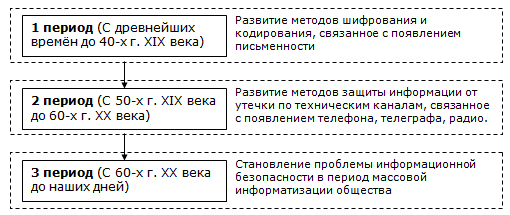
\includegraphics[width=\linewidth]{pr1_1}
  \caption{Периоды развития}\label{pr1_1}
\end{figure}

Наблюдаемые в последние годы тенденции в развитии информационных технологий
могут уже в недалеком будущем привести к появлению качественно новых
(информационных) форм борьбы, в том числе и на межгосударственном уровне,
которые могут принимать форму информационной войны, а сама информационная
война станет одним из основных инструментов внешней политики, включая защиту
государственных интересов и реализацию любых форм агрессии. Это является
одной из причин, почему полезно ознакомиться с основными принципами
обеспечения ИБ в ведущих зарубежных странах.

Прежде чем говорить об обеспечении безопасности персональных данных,
необходимо определить, что же такое информационная безопасность. Термин
<<информационная безопасность>> может иметь различный смысл и трактовку в
зависимости от контекста. В данном пособии под информационной безопасностью
мы будем понимать защищённость информации и поддерживающей инфраструктуры от
случайных или преднамеренных воздействий естественного или искусственного
характера, которые могут нанести неприемлемый ущерб субъектам информационных
отношений, в том числе владельцам и пользователям информации и поддерживающей
инфраструктуры.\href{https://www.intuit.ru/studies/courses/697/553/literature#literature.1}{\todo{[1]}}

\textbf{Информационная безопасность}~---~это защищённость информации и
поддерживающей её инфраструктуры от случайных или преднамеренных воздействий
естественного или искусственного характера, которые могут нанести ущерб
владельцам или пользователям информации.

В ряде случаев понятие <<информационная безопасность>> подменяется термином
<<компьютерная безопасность>>. В этом случае информационная безопасность
рассматривается очень узко, поскольку компьютеры только одна из составляющих
информационных систем. Несмотря на это, в рамках изучаемого курса основное
внимание будет уделяться изучению вопросов, связанных с обеспечением режима
информационной безопасности применительно к вычислительным системам, в
которых информация хранится, обрабатывается и передаётся с помощью
компьютеров. Согласно определению, компьютерная безопасность зависит не
только от компьютеров, но и от поддерживающей инфраструктуры, к которой можно
отнести системы электроснабжения, жизнеобеспечения, вентиляции, средства
коммуникаций, а также обслуживающий персонал.


\subsection{Составляющие информационной безопасности}%
Обеспечение информационной безопасности в большинстве случаев связано с
комплексным решением трёх задач:
\begin{Notes}
  \item \textbf{Конфиденциальность} – состояние информации, при котором
      доступ к ней осуществляют только субъекты, имеющие на него право.
  \item \textbf{Целостность} – состояние информации, при котором
      отсутствует любое её изменение либо изменение осуществляется только
      преднамеренно субъектами, имеющими на него право;
  \item \textbf{Доступность} – состояние информации, при котором субъекты,
      имеющие право доступа, могут реализовывать его беспрепятственно.
\end{Notes}

\textbf{Угрозы информационной безопасности}~---~совокупность условий и
факторов, создающих потенциальную или реально существующую опасность
нарушения безопасности информации.
\href{https://www.intuit.ru/studies/courses/697/553/literature#literature.1}{[2,3]}

\textbf{Атака}~---~это попытка реализации угрозы. Кто предпринимает такую
попытку, называется \textbf{злоумышленником}. Потенциальные злоумышленники
называются \textbf{источниками угрозы}.

Угроза является следствием наличия уязвимых мест или уязвимости в
информационной системе. Уязвимости могут возникать по разным причинам,
например, в результате непреднамеренных ошибок программистов при написании
программ.

\noindent Угрозы можно классифицировать по нескольким критериям:
\begin{itemize}
  \item по свойствам информации (доступность, целостность,
      конфиденциальность), против которых угрозы направлены в первую
      очередь;
  \item по компонентам информационных систем, на которые угрозы нацелены
      (данные, программы, аппаратура, поддерживающая инфраструктура);
  \item по способу осуществления (случайные/преднамеренные, действия
      природного/техногенного характера);
  \item по расположению источника угроз (внутри/вне рассматриваемой ИС).
\end{itemize}
Обеспечение информационной безопасности является сложной задачей, для решения
которой требуется комплексный подход.

\subsection{Уровни защиты информации}
\subsubsection{Законодательный уровень}
Законодательный уровень является основой для построения системы защиты
информации, так как даёт базовые понятия предметной области и определяет меру
наказания для потенциальных злоумышленников. Этот уровень играет
координирующую и направляющую роли и помогает поддерживать в обществе
негативное (и карательное) отношение к людям, нарушающим информационную
безопасность.

Законодательно-правовой уровень включает комплекс законодательных и иных
правовых актов, устанавливающих правовой статус субъектов информационных
отношений, субъектов и объектов защиты, методы, формы и способы защиты, их
правовой статус. Кроме того, к этому уровню относятся стандарты и
спецификации в области информационной безопасности. Система законодательных
актов и разработанных на их базе нормативных и
организационно-распорядительных документов должна обеспечивать организацию
эффективного надзора за их исполнением со стороны правоохранительных органов
и реализацию мер судебной защиты и ответственности субъектов информационных
отношений. К этому уровню можно отнести и морально-этические нормы поведения,
которые сложились традиционно или складываются по мере распространения
вычислительных средств в обществе. Морально-этические нормы могут быть
регламентированными в законодательном порядке, т. е. в виде свода правил и
предписаний. Наиболее характерным примером таких норм является Кодекс
профессионального поведения членов Ассоциации пользователей ЭВМ США. Тем не
менее, эти нормы большей частью не являются обязательными, как
законодательные меры.
\subsubsection{Административный уровень}
Это комплекс мер, предпринимаемых локально руководством организации. Включает
комплекс взаимокоординируемых мероприятий и технических мер, реализующих
практические механизмы защиты в процессе создания и эксплуатации систем
защиты информации. Организационный уровень должен охватывать все структурные
элементы систем обработки данных на всех этапах их жизненного цикла:
строительство помещений, проектирование системы, монтаж и наладка
оборудования, испытания и проверки, эксплуатация.

Разработка политики безопасности - дело тонкое, поскольку у каждой
организации есть своя специфика. Здесь бессмысленно переносить практику
режимных государственных организаций на коммерческие структуры, учебные
заведения или персональные компьютерные системы. В этой области целесообразно
предложить, во-первых, основные принципы разработки политики безопасности, а,
во-вторых, - готовые шаблоны для наиболее важных разновидностей организаций.
\subsubsection{Процедурный уровень}
К процедурному уровню относятся меры безопасности, реализуемые людьми. В
отечественных организациях накоплен богатый опыт составления и реализации
процедурных (организационных) мер, однако проблема состоит в том, что они
пришли из докомпьютерного прошлого, поэтому нуждаются в существенном
пересмотре.

\noindent Можно выделить следующие группы процедурных мер:
\begin{itemize}
 \item управление персоналом;%
 \item физическая защита;%
 \item поддержание работоспособности;%
 \item реагирование на нарушения режима безопасности;%
 \item планирование восстановительных работ.%
\end{itemize}
Для каждой группы в каждой организации должен существовать набор регламентов,
определяющих действия персонала. В свою очередь, исполнение этих регламентов
следует отработать на практике.
\subsubsection{Программно-технический уровень}
Согласно современным воззрениям, включает три подуровня: физический,
технический (аппаратный) и программный.

Физический подуровень решает задачи с ограничением физического доступа к
информации и информационным системам, соответственно к нему относятся
технические средства, реализуемые в виде автономных устройств и систем, не
связанных с обработкой, хранением и передачей информации: система охранной
сигнализации, система наблюдения, средства физического воспрепятствования
доступу (замки, ограждения, решётки и т. д.).

Средства защиты аппаратного и программного подуровней непосредственно связаны
с системой обработки информации. Эти средства либо встроены в аппаратные
средства обработки, либо сопряжены с ними по стандартному интерфейсу.К
аппаратным средствам относятся схемы контроля информации по четности, схемы
доступа по ключу и т. д.

К программным средствам защиты, образующим программный подуровень, относятся
специальное программное обеспечение, используемое для защиты информации,
например антивирусный пакет и т. д. Программы защиты могут быть как
отдельные, так и встроенные. Подчеркнём, что формирование режима
информационной безопасности является сложной системной задачей, решение
которой в разных странах отличается по содержанию и зависит от таких
факторов, как научный потенциал страны, степень внедрения средств
информатизации в жизнь общества и экономику, развитие производственной базы,
общей культуры общества и, наконец, традиций и норм поведения.

\subsection{Виды информационных угроз}
\noindent Информационные угрозы могут быть обусловлены:
\begin{itemize}[noitemsep]
  \item естественными факторами (пожар, наводнение, и др.);
  \item человеческими факторами.
\end{itemize}
\noindent Последние, в свою очередь, подразделяются на:
\begin{Notes}
  \item Угрозы, носящие случайный, неумышленный характер. Это
      угрозы, связанные с ошибками процесса подготовки, обработки и
      передачи информации;
  \item Угрозы, обусловленные умышленными, преднамеренными
      действиями людей. Это угрозы, связанные с несанкционированным
      доступом к ресурсам АИС.
\end{Notes}
Умышленные угрозы преследуют цель нанесения ущерба пользователям АИС и, в
свою очередь, подразделяются на активные и пассивные. Угрозы также
подразделяются на внутренние, возникающие внутри управляемой организации, и
внешние.

\emph{Под внутренними угрозами понимаются}~---~угрозы безопасности информации
инсайдером (исполнителем) которых является внутренний по отношению к ресурсам
организации субъект (инсайдер).

\emph{Под внешними угрозами понимаются}~---~угрозы безопасности информации
инициатором (исполнителем) которых является внешний по отношению к ресурсам
организации субъект (удаленный хакер, злоумышленник).



\section{Практические задания}\label{sect1_b}

\subsection{Тестирование}\label{sect1_b_1}
%
\begin{enumerate}
  \item В чем заключается проблема информационной безопасности?
  \item Дайте определение понятию <<информационная безопасность>>.
  %\item Какие определения информационной безопасности приводятся в
  %    "Концепции информационной безопасности сетей связи общего пользования
  %    Российской Федерации"?
  \item Что понимается под <<компьютерной безопасностью>>?
  \item Перечислите составляющие информационной безопасности.
  \item Приведите определение доступности информации.
  \item Приведите определение целостности информации.
  \item Приведите определение конфиденциальности информации.
  \item Каким образом взаимосвязаны между собой составляющие информационной
      безопасности? Приведите собственные примеры.
  \item Перечислите задачи информационной безопасности общества.
  \item Перечислите уровни формирования режима информационной безопасности.
  \item Дайте краткую характеристику законодательно-правового уровня.
  \item Какие подуровни включает программно-технический уровень?
  \item Что включает административный уровень?
  \item В чем особенность морально-этического подуровня?
\end{enumerate}

\subsection{Разбор ситуации}
В данной части практического задания следует оценить актуальность,
возможность и критичность угроз. Оценив всю необходимую информацию и взвесив
все <<за>> и <<против>>.

В дополнение следует подобрать наиболее оптимальные методы и средства защиты.

\href{https://habrahabr.ru/company/vps_house/blog/343110/}{Первая часть
      статьи}

\label{var_PR1}
\begin{minipage}{0.45\textwidth}
  \begin{enumerate}
    \item Отделение коммерческого банка;
    \item Поликлиника;
    \item Колледж;
    \item Офис страховой компании;
    \item Рекрутинговое агентство;
    \item Интернет-магазин;
    \item Центр оказания гос. услуг;
    \item Отделение полиции;
    \item Аудиторская компания;
    \item Дизайнерская фирма;
    \item Офис интернет-провайдера;
    \item Офис адвоката;
    \item Компания по разработке ПО;
    \item Агентство недвижимости;
    \item Туристическое агентство;
  \end{enumerate}
\end{minipage}
\hfill
\begin{minipage}{0.45\textwidth}
  \begin{enumerate}
    \setcounter{enumi}{15}
    \item Офис благотворительного фонда;
    \item Издательство;
    \item Консалтинговая фирма;
    \item Рекламное агентство;
    \item Отделение налоговой службы;
    \item Офис нотариуса;
    \item Бюро перевода (документов);
    \item Научно проектное предприятие;
    \item Брачное агентство;
    \item Редакция газеты;
    \item Гостиница;
    \item Праздничное агентство;
    \item Городской архив;
    \item Диспетчерская служба такси;
    \item Железнодорожная касса.
  \end{enumerate}
\end{minipage}

 %\begin{enumerate}
 %  \item Сотрудница бухгалтерского отделения разместила фото с id своей
 %      карты в социальной сети.
 %  \item Подкуплен сотрудник, в результате чего в здание главного офиса
 %      проник неизвестный человек.
 %  \item Сильный ливень повредил обшивку здания и проник в серверную, в
 %      результате компания вышла из рынка на пару суток и потерей множества
 %      данных из личного архива.
 %  \item Вирус проникший в ПК одного из сотрудников распространился по всей
 %      компании.
 %  \item В результате попадения вируса были повреждены данные на права
 %      использования продуктов в фирме.
 %  \item Из-за перебоев в работе сети организация теряет клиентов.
 %  \item Зафиксирован взлом шифра передачи информации между отделами офиса.
 %  \item При пожаре в здании были уничтожены ценные бумаги.
 %  \item При подкупе сотрудника структура была систематически
 %      дезинформирована.
 %  \item При сбоях в работе межсетевого экрана компания потеряла
 %      защищённость сети.
 %  \item Внедрение <<троянского коня>> в систему, периодическое
 %      прослушивание эфира.
 %  \item Искажение информации путём подкупа персонала.
 %  \item Удаление информации сотрудником при неправильном использовании ПО.
 %  \item - -- ---
 %  \item (Авария, ошибка пользователя, привели к угрозам в безопасности
 %      информационного ресурса)
 %  \item (Отказ аппаратного обеспечения, доступ к веб-ресурсу для персонала)
 %  \item (Хакер нарушил конфидециальность данных используя ошибку
 %      администратора)
 %  \item (В связи с несоблюдением мер безопасности нарушена
 %      конфиденциальность личных данных персонала)
 %  \item ( Произведён несанкционированный доступ в сети неавторизованным
 %      пользователем)
 %  \item (Ошибка хранения данных)
 %  \item разглашение секретной информации после увольнения сотрудника
 %  \item преднамеренный взрыв в здании,  потеря текущих трансакций компании
 %  \item Нарушена целостность данных путём взлома одного из удалённых
 %      сервисов компании.
 %  \item Нарушение от установленных правил эксплуатации оборудования.
 %  \item Ошибка при переконфигурировании системы временным сотрудником.
 %  \item дублирование данных компании сотрудником на флеш накопитель.
 %  \item Сбой в работе компании по обеспечению vps серверов.
 %  \item
 %\end{enumerate}

\chapter{Методы защиты информации} \label{chapt2}%
\textbf{Мета роботи:~}%
На практике использовать основные методы криптографической зашиты информации.
\section{Теоретические ведомости} \label{sect8_a}
%
Появление новых информационных технологий и развитие мощных компьютерных
систем хранения и обработки информации повысили уровни защиты информации и
вызвали необходимость того, чтобы эффективность защиты информации росла
вместе со сложностью архитектуры хранения данных. Постепенно защита
информации становится обязательной: разрабатываются всевозможные документы по
защите информации; формируются рекомендации; даже проводится ФЗ о защите
информации, который рассматривает проблемы и задачи защиты информации, а
также решает некоторые уникальные вопросы защиты информации.

Таким образом, угроза защиты информации сделала средства обеспечения
информационной безопасности одной из обязательных характеристик
информационной системы.

\begin{figure}[h]
  \centering
  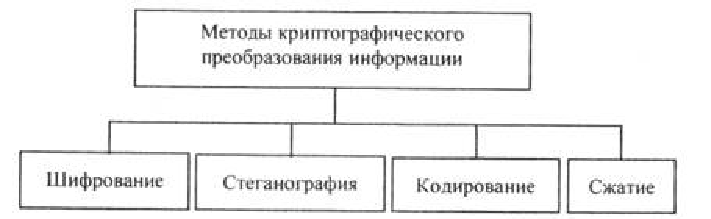
\includegraphics[width=\linewidth]{img2_1.pdf}
  \caption{Методы криптографического преобразования информации}\label{img:img2_1}
\end{figure}



\subsection{Симметричные криптосистемы}
\subsubsection{Шифры перестановки}
В шифрах средних веков часто использовались таблицы, с помощью которых
выполнялись простые процедуры шифрования, основанные на перестановке букв в
сообщении. Ключом в данном случае является размеры таблицы. Например,
сообщение <<Неясное становится ещё более непонятным>> записывается в таблицу
из 5 строк и 7 столбцов по столбцам.

\begin{table} [htbp]% Пример записи таблицы с номером, но без отображаемого наименования
  \centering
  \parbox{6cm}{% чтобы лучше смотрелось, подбирается самостоятельно
    \captiondelim{}% должен стоять до самого пустого caption
    \caption{}%
    \label{tabl:tab2x1}%
    \begin{SingleSpace}
      \begin{tabular}{ | c | c | c | c | c | c | c |}
        \hline
          Н & О & Н & С & Б & Н & Я \\ \hline
          Е & Е & О & Я & О & Е & Т \\ \hline
          Я & С & В & Е & Л & П & Н \\ \hline
          С & Т & И & Щ & Е & О & Ы \\ \hline
          Н & А & Т & Ё & Е & Н & М \\ \hline
      \end{tabular}%
    \end{SingleSpace}
  }
\end{table}
Для получения шифрованного сообщения текст считывается по строкам и
группируется по 5 букв:
\begin{center}
НОНСБ--НЯЕЕО--ЯОЕТЯ--СВЕЛП--НСТИЩ--ЕОЫНА--ТЕЕНМ
\end{center}

Несколько большей стойкостью к раскрытию обладает метод \emph{одиночной
перестановки} по ключу. Он отличается от предыдущего тем, что столбцы таблицы
переставляются по ключевому слову, фразе или набору чисел длиной в строку
таблицы. Используя в качестве ключа слово - \texttt{ЛУНАТИК}, получим
следующую таблицу:

\begin{table} [htbp]% Пример записи таблицы с номером, но без отображаемого наименования
  \centering
  \parbox{12cm}%
  {% чтобы лучше смотрелось, подбирается самостоятельно
    \caption{Метод перестановки по ключу}%
    \label{tabl:tab2x2}%
    \begin{SingleSpace}
      \begin{tabular}{ccccccccccccccc}
      \cline{1-7} \cline{9-15}
      \multicolumn{1}{|c|}{{\ul Л}}    & \multicolumn{1}{c|}{{\ul У}}    & \multicolumn{1}{c|}{{\ul Н}}    & \multicolumn{1}{c|}{{\ul А}}    & \multicolumn{1}{c|}{{\ul Т}}    & \multicolumn{1}{c|}{{\ul И}}    & \multicolumn{1}{c|}{{\ul К}}    & \multicolumn{1}{c|}{} & \multicolumn{1}{c|}{{\ul А}}    & \multicolumn{1}{c|}{{\ul И}}    & \multicolumn{1}{c|}{{\ul К}}    & \multicolumn{1}{c|}{{\ul Л}}    & \multicolumn{1}{c|}{{\ul Н}}    & \multicolumn{1}{c|}{{\ul Т}}    & \multicolumn{1}{c|}{{\ul У}}    \\ \cline{1-7} \cline{9-15}
      \multicolumn{1}{|c|}{\textbf{4}} & \multicolumn{1}{c|}{\textbf{7}} & \multicolumn{1}{c|}{\textbf{5}} & \multicolumn{1}{c|}{\textbf{1}} & \multicolumn{1}{c|}{\textbf{6}} & \multicolumn{1}{c|}{\textbf{2}} & \multicolumn{1}{c|}{\textbf{3}} & \multicolumn{1}{c|}{} & \multicolumn{1}{c|}{\textbf{1}} & \multicolumn{1}{c|}{\textbf{2}} & \multicolumn{1}{c|}{\textbf{3}} & \multicolumn{1}{c|}{\textbf{4}} & \multicolumn{1}{c|}{\textbf{5}} & \multicolumn{1}{c|}{\textbf{6}} & \multicolumn{1}{c|}{\textbf{7}} \\ \cline{1-7} \cline{9-15}
      \multicolumn{1}{|c|}{Н}          & \multicolumn{1}{c|}{О}          & \multicolumn{1}{c|}{Н}          & \multicolumn{1}{c|}{С}          & \multicolumn{1}{c|}{Б}          & \multicolumn{1}{c|}{Н}          & \multicolumn{1}{c|}{Я}          & \multicolumn{1}{c|}{} & \multicolumn{1}{c|}{С}          & \multicolumn{1}{c|}{Н}          & \multicolumn{1}{c|}{Я}          & \multicolumn{1}{c|}{Н}          & \multicolumn{1}{c|}{Н}          & \multicolumn{1}{c|}{Б}          & \multicolumn{1}{c|}{О}          \\ \cline{1-7} \cline{9-15}
      \multicolumn{1}{|c|}{Е}          & \multicolumn{1}{c|}{Е}          & \multicolumn{1}{c|}{О}          & \multicolumn{1}{c|}{Я}          & \multicolumn{1}{c|}{О}          & \multicolumn{1}{c|}{Е}          & \multicolumn{1}{c|}{Т}          & \multicolumn{1}{c|}{} & \multicolumn{1}{c|}{Я}          & \multicolumn{1}{c|}{Е}          & \multicolumn{1}{c|}{Т}          & \multicolumn{1}{c|}{Е}          & \multicolumn{1}{c|}{О}          & \multicolumn{1}{c|}{О}          & \multicolumn{1}{c|}{Е}          \\ \cline{1-7} \cline{9-15}
      \multicolumn{1}{|c|}{Я}          & \multicolumn{1}{c|}{С}          & \multicolumn{1}{c|}{В}          & \multicolumn{1}{c|}{Е}          & \multicolumn{1}{c|}{Л}          & \multicolumn{1}{c|}{П}          & \multicolumn{1}{c|}{Н}          & \multicolumn{1}{c|}{} & \multicolumn{1}{c|}{Е}          & \multicolumn{1}{c|}{П}          & \multicolumn{1}{c|}{Н}          & \multicolumn{1}{c|}{Я}          & \multicolumn{1}{c|}{В}          & \multicolumn{1}{c|}{Л}          & \multicolumn{1}{c|}{С}          \\ \cline{1-7} \cline{9-15}
      \multicolumn{1}{|c|}{С}          & \multicolumn{1}{c|}{Т}          & \multicolumn{1}{c|}{И}          & \multicolumn{1}{c|}{Щ}          & \multicolumn{1}{c|}{Е}          & \multicolumn{1}{c|}{О}          & \multicolumn{1}{c|}{Ы}          & \multicolumn{1}{c|}{} & \multicolumn{1}{c|}{Щ}          & \multicolumn{1}{c|}{О}          & \multicolumn{1}{c|}{Ы}          & \multicolumn{1}{c|}{С}          & \multicolumn{1}{c|}{И}          & \multicolumn{1}{c|}{Е}          & \multicolumn{1}{c|}{Т}          \\ \cline{1-7} \cline{9-15}
      \multicolumn{1}{|c|}{Н}          & \multicolumn{1}{c|}{А}          & \multicolumn{1}{c|}{Т}          & \multicolumn{1}{c|}{Е}          & \multicolumn{1}{c|}{Е}          & \multicolumn{1}{c|}{Н}          & \multicolumn{1}{c|}{М}          & \multicolumn{1}{c|}{} & \multicolumn{1}{c|}{Е}          & \multicolumn{1}{c|}{Н}          & \multicolumn{1}{c|}{М}          & \multicolumn{1}{c|}{Н}          & \multicolumn{1}{c|}{Т}          & \multicolumn{1}{c|}{Е}          & \multicolumn{1}{c|}{А}          \\ \cline{1-7} \cline{9-15}
      \multicolumn{7}{c}{До перестановки}                                                                                                                                                                                                          & \multicolumn{1}{l}{}  & \multicolumn{7}{c}{После перестановки}
      \end{tabular}
    \end{SingleSpace}
  }
\end{table}

В верхней строке левой таблицы записан ключ, а номера под буквами ключа
определены в соответствии с естественным порядком соответствующих букв ключа
в алфавите. Если в ключе встретились бы одинаковые буквы, они бы нумеровались
слева направо. Получается шифровка:%
\begin{center}
СНЯНН--БОЯЕТ--ЕООЕЕ--ПНЯВЛ--СЩОЫС--ИЕТЕН--МНТЕА
\end{center}

Для обеспечения дополнительной скрытности можно повторно шифровать сообщение,
которое уже было зашифровано. Для этого размер второй таблицы подбирают так,
чтобы длины её строк и столбцов отличались от длин строк и столбцов первой
таблицы. Лучше всего, если они будут взаимно простыми.

Кроме алгоритмов одиночных перестановок применяются алгоритмы двойных
перестановок. Сначала в таблицу записывается текст сообщения, а потом
поочередно переставляются столбцы, а затем строки. При расшифровке порядок
перестановок был обратный. Пример данного метода шифрования показан в таблице
\ref{tabl:tab2x3}.

\begin{table} [htbp]% Пример записи таблицы с номером, но без отображаемого наименования
  \centering
  \parbox{12cm}{% чтобы лучше смотрелось, подбирается самостоятельно
    \caption{Метод перестановки по ключу}%
    \label{tabl:tab2x3}%
    \begin{SingleSpace}
      \begin{tabular}{c|c|c|c|c|cc|c|c|c|c|cc|c|c|c|c|}
      \cline{2-5} \cline{8-11} \cline{14-17}
      \textbf{}                        & \textbf{2}                                                & \textbf{4} & \textbf{1} & \textbf{3}                                                &                       & \textbf{} & {\color[HTML]{00FE00} \textbf{1}} & {\color[HTML]{00FE00} \textbf{2}}                         & {\color[HTML]{00FE00} \textbf{3}}                         & {\color[HTML]{00FE00} \textbf{4}} &                       &                                   & 1 & 2                                                         & 3                                                         & 4 \\ \cline{1-5} \cline{7-11} \cline{13-17}
      \multicolumn{1}{|c|}{\textbf{4}} & \cellcolor[HTML]{ECF4FF}{\color[HTML]{000000} \textbf{П}} & Р          & И          & Е                                                         & \multicolumn{1}{c|}{} & 4         & И                                 & \cellcolor[HTML]{ECF4FF}{\color[HTML]{000000} \textbf{П}} & Е                                                         & Р                                 & \multicolumn{1}{c|}{} & {\color[HTML]{FE0000} \textbf{1}} & А & З                                                         & Ю                                                         & Ж \\ \cline{1-5} \cline{7-11} \cline{13-17}
      \multicolumn{1}{|c|}{\textbf{1}} & З                                                         & Ж          & А          & Ю                                                         & \multicolumn{1}{c|}{} & 1         & А                                 & 3                                                         & Ю                                                         & Ж                                 & \multicolumn{1}{c|}{} & {\color[HTML]{FE0000} \textbf{2}} & Е & -                                                         & С                                                         & Ш \\ \cline{1-5} \cline{7-11} \cline{13-17}
      \multicolumn{1}{|c|}{\textbf{2}} & -                                                         & Ш          & Е          & С                                                         & \multicolumn{1}{c|}{} & 2         & Е                                 & -                                                         & С                                                         & Ш                                 & \multicolumn{1}{c|}{} & {\color[HTML]{FE0000} \textbf{3}} & Г & Т                                                         & \cellcolor[HTML]{ECF4FF}{\color[HTML]{000000} \textbf{О}} & О \\ \cline{1-5} \cline{7-11} \cline{13-17}
      \multicolumn{1}{|c|}{\textbf{3}} & Т                                                         & О          & Г          & \cellcolor[HTML]{ECF4FF}{\color[HTML]{000000} \textbf{О}} & \multicolumn{1}{c|}{} & 3         & Г                                 & Т                                                         & \cellcolor[HTML]{ECF4FF}{\color[HTML]{000000} \textbf{О}} & О                                 & \multicolumn{1}{c|}{} & {\color[HTML]{FE0000} \textbf{4}} & И & \cellcolor[HTML]{ECF4FF}{\color[HTML]{000000} \textbf{П}} & Е                                                         & Р \\ \cline{1-5} \cline{7-11} \cline{13-17}
      \end{tabular}
    \end{SingleSpace}
  }
\end{table}
Ключом к шифру служат номера столбцов \textbf{\textcolor[rgb]{0,1,0}{2413}} и
номера строк \textbf{\textcolor[rgb]{1,0,0}{4123}} исходной таблицы. В
результате перестановки получена шифровка:
\begin{center}
АЗЮЖЕ\_СШГТООИПЕР
\end{center}
Число вариантов двойной перестановки достаточно быстро возрастает с
увеличением размера таблицы: для таблицы $3 х 3$ их $36$, для $4 х 4$ их
$576$, а для $5\cdot 5$ их $14400$.

В средние века для шифрования применялись и магические квадраты. Магическими
квадратами называются квадратные таблицы с вписанными в их клетки
последовательными натуральными числами, начиная с единицы, которые дают в
сумме по каждому столбцу, каждой строке и каждой диагонали одно и то же
число. Для шифрования необходимо вписать исходный текст по приведённой в
квадрате нумерации и затем переписать содержимое таблицы по строкам.
\begin{table} [htbp]% Пример записи таблицы с номером, но без отображаемого наименования
  \centering
  \parbox{14cm}{% чтобы лучше смотрелось, подбирается самостоятельно
    \caption{Исходный текст с идентификаторами}%
    \label{tabl:tab2x4}%
    \begin{SingleSpace}
\begin{tabular}{c|c|c|c|c|c|c|c|c|c|c|c|c|c|c|c}
П & Р & И & Е & З & Ж & А & Ю & \_ & Ш & Е & С & Т & О & Г & О \\ \hline
1 & 2 & 3 & 4 & 5 & 6 & 7 & 8 & 9 & 10 & 11 & 12 & 13 & 14 & 15 & 16 \\
\end{tabular}
    \end{SingleSpace}
  }
\end{table}
\begin{table}% Пример записи таблицы с номером, но без отображаемого наименования
  \centering
  \parbox{10cm}{% чтобы лучше смотрелось, подбирается самостоятельно
    \caption{Магический квадрат}%
    \label{tabl:tab2x5}%
    \begin{SingleSpace}
      \begin{tabular}{|c|c|c|c|c|c|c|c|c|}
\cline{1-4} \cline{6-9}
16 & 3  & 2  & 13 &                     & О & И & Р & Т \\ \cline{1-4} \cline{6-9}
5  & 10 & 11 & 8  & {\Huge $\dashrightarrow$} & З & Ш & Е & Ю \\ \cline{1-4} \cline{6-9}
9  & 6  & 7  & 12 & {\Huge $\dashleftarrow$}  & - & Ж & А & С \\ \cline{1-4} \cline{6-9}
4  & 15 & 14 & 1  &                     & Е & Г & О & П \\ \cline{1-4} \cline{6-9}
      \end{tabular}
    \end{SingleSpace}
  }
\end{table}
В результате получается шифротекст, сформированный благодаря перестановке
букв исходного сообщения.

Число магических квадратов очень резко возрастает с увеличением размера его
сторон: для таблицы $3\times 3~\Rightarrow~1$ существует только один квадрат;
для таблицы $4\times 4~\Rightarrow~880$; а для таблицы $5\times
5~\Rightarrow~250 000$.


\subsubsection{Шифры простой замены}

\subparagraph{Система шифрования Цезаря} частный случай шифра простой замены.
Метод основан на замене каждой буквы сообщения на другую букву того же
алфавита, путем смещения от исходной буквы на \emph{K} букв. Известная фраза
Юлия Цезаря \texttt{VENI VINI VICI} – пришел, увидел, победил, зашифрованная
с помощью данного метода, преобразуется в \texttt{SBKF SFAF SFZF} (при
смещении на 4 символа). Греческим писателем Полибием за 100 лет до н.э. был
изобретён так называемый полибианский квадрат размером $5\times 5$,
заполненный алфавитом в случайном порядке. Греческий алфавит имеет 24 буквы,
а 25-м символом является пробел. Для шифрования на квадрате находили букву
текста и записывали в шифротекст букву, расположенную ниже её в том же
столбце. Если буква оказывалась в нижней строке таблицы, то брали верхнюю
букву из того же столбца.

\subsubsection{Шифры сложной замены}

\subparagraph{Шифр Гронсфельда} состоит в модификации шифра Цезаря числовым
ключом. Для этого под буквами сообщения записывают цифры числового ключа.
Если ключ короче сообщения, то его запись циклически повторяют. Шифротекст
получают примерно так же, как в шифре Цезаря, но отсчитывают не третью букву
по алфавиту (как в шифре Цезаря), а ту, которая смещена по алфавиту на
соответствующую цифру ключа.
\begin{Notes}
  \item пусть в качестве ключа используется группа из трех цифр - 314;
  \item тогда Сообщение СОВЕРШЕННО СЕКРЕТНО;
  \item Ключ 3143143143143143143;
  \item Шифровка ФПЖИСЬИОССАХИЛФИУСС.
\end{Notes}
В шифрах \emph{многоалфавитной замены} для шифрования каждого символа
исходного сообщения применяется свой шифр простой замены (свой алфавит).

В компьютере операция шифрования соответствует сложению кодов ASCII символов
сообщения и ключа по модулю 256.

\subsubsection{Гаммирование}
Процесс зашифрования заключается в генерации гаммы шифра и наложении этой
гаммы на исходный открытый текст. Перед шифрованием открытые данные
разбиваются на блоки $T(0)_i$ одинаковой длины (по 64 бита). Гамма шифра
вырабатывается в виде последовательности блоков Г(c)i аналогичной длины
$Т(c)_i=G(c)_i \oplus T(0)_i$, где $\oplus $ - побитовое сложение, $i =1-m$).

Процесс расшифрования сводится к повторной генерации шифра текста и наложение
этой гаммы на зашифрованные данные $T(0)_i=G(c)_i\oplus Т(c)_i$.

Исходное сообщение из букв русского алфавита преобразуется в числовое
сообщение заменой каждой его буквы числом по следующей таблице:


\begin{table}[htbp]% Пример записи таблицы с номером, но без отображаемого наименования
  \centering
  \caption{Числовая замена букв}%
  \label{tabl:tab2x6}%
    \begin{SingleSpace}
    \begin{tabularx}{\textwidth}{|C|C|C|C|C|C|C|C|C|C|C|C|C|C|C|}
      \hline
      А  & Б  & В  & Г  & Д  & Е  & Ж  & З  & И  & К  & Л  & М  & Н  & О  & П  \tabularnewline \hline
      00 & 01 & 02 & 03 & 04 & 05 & 06 & 07 & 08 & 09 & 10 & 11 & 12 & 13 & 14 \tabularnewline \hline
      Р  & С  & Т  & У  & Ф  & Х  & Ц  & Ч  & Ш  & Щ  & Ь  & Ы  & Э  & Ю  & Я  \tabularnewline \hline
      15 & 16 & 17 & 18 & 19 & 20 & 21 & 22 & 23 & 24 & 25 & 26 & 27 & 28 & 29 \tabularnewline \hline
      \end{tabularx}
  \end{SingleSpace}
\end{table}
\begin{equation}\label{formul:fml2_1}
  {\Omega}_{i+1}= [(A_i + C_1 – 1)\cdot mod30] + 1;
\end{equation}

Исходное сообщение ОТДУШКА. Для шифрования числового сообщения используется
шифрующий отрезок последовательности А1, А2, ... подходящей длины,
начинающийся с $A_{100}$: $A_{101}\rightarrow 5$, $A_{102}\rightarrow 6$,
$A_{103}\rightarrow 17$, $A_{104}\rightarrow 18$, $A_{105}\rightarrow 19$,
$A_{106}\rightarrow 3$.

\begin{table}[htbp]% Пример записи таблицы с номером, но без отображаемого наименования
  \centering
    \captiondelim{}% должен стоять до самого пустого caption
  %\caption{}%caption{Пример шифрования методом гаммирование}%
  \label{tabl:tab2x7}%
  \begin{tabular}{lccccccc}
    Исходное сообщение             & О  & Т  & Д  & У  & Ш  & К  & А \\
    \rowcolor[HTML]{EFEFEF}
    Числовое исходное сообщение    & 13 & 17 & 4  & 18 & 23 & 9  & 0 \\
    Шифрующий отрезок              & 1  & 5  & 6  & 17 & 8  & 19 & 3 \\
    \rowcolor[HTML]{EFEFEF}
    Числовое шифрованное сообщение & 14 & 23 & 10 & 5  & 1  & 28 & 3 \\
    Шифрованное сообщение          & П  & Ш  & Л  & Е  & Б  & Ю  & Г
  \end{tabular}
\end{table}

\section{Задания}\label{sect8_b}
%
(из заданий к экзамену)
\section{Пример выполнения работы}\label{sect8_c}
%
\section{Варианты}\label{sect8_d}
%
\section{Вопросы для контроля}\label{sect8_e}
%
\begin{enumerate}
  \item
  \item
  \item
\end{enumerate}

\chapter{Методы атаки. Частотная атака} \label{chapt3}%
\textbf{Мета роботи:~}%
Изучение способов атаки на разные уровни системы. Методы подбора и анализ
частотной атаки.
\section{Теоретические ведомости} \label{sect2_a}
%
\textbf{Моноалфавитный подстановочный шифр} -- шифр, в котором каждой букве
исходного алфавита поставлена в соответствие одна буква шифра.


Например, возьмем слово \texttt{КУКУРУЗА}. Пусть букве \texttt{К} текста
соответствует буква \texttt{А} шифра, букве \texttt{У} текста соответствует
буква \texttt{Б} шифра, букве \texttt{Р} текста соответствует буква
\texttt{В} шифра, букве \texttt{З} текста соответствует буква \texttt{Г}
шифра, букве \texttt{А} текста соответствует буква \texttt{Д} шифра. После
подстановки букв шифра вместо букв исходного теста слово \texttt{КУКУРУЗА} в
зашифрованном виде будет выглядеть как \texttt{АБАБВБГД}. Недостатком
подобного шифрования является то, что, если какая-то буква встречается в
исходном тексте чаще всего (например, буква \texttt{О} в русском алфавите),
то и соответствующая ей буква шифра в зашифрованном тексте также встречается
чаще всего. В ниже приведенной таблице приведены частоты встречаемости букв в
английском тексте (в процентах):

\todo{диаграмма частот использования букв алфавита}

Зная частоты наиболее встречающихся букв и подсчитав, какие буквы чаще всего
встречаются в шифровке, криптоаналитик может подобрать расшифровку для
некоторых букв текста. Затем, анализируя короткие слова, найти еще буквы,
истинные значения которых можно с высокой степенью уверенности предугадать.
Например, если уже расшифрована    буква    \texttt{О}    и    в    тексте
есть слово    \texttt{ОЫО}    (подчеркнуты  уже расшифрованные буквы), то,
скорее всего, шифру \texttt{Ы} соответствует буква \texttt{Н} в исходном
тексте (\texttt{ОНО}). Чем дальше расшифровывается текст, тем легче идет
процесс расшифровки.


\section{Задания}\label{sect2_b}
%
\begin{enumerate}
  \item Освоить теорию и принципы частотной атаки.
  \item Проанализировать представленное ПО
  \item Расшифровать текст и предоставить: %
  \begin{itemize}
    \item шифрованное сообщение;
    \item перечень замен;
    \item расшифрованный текст;
    \item предоставить алгоритм дешифровки\footnote{Задание для
        дополнительных баллов.}.
  \end{itemize}
  \item Выводы к работе
\end{enumerate}
\section{Пример выполнения работы}\label{sect2_c}
%
\section{Варианты}\label{sect2_d}
%
\section{Вопросы для контроля}\label{sect2_e}
%

\chapter{Построение концепции информационной безопасности предприятия} \label{chapt4}%
\textbf{Мета роботи:~}%
Знакомство с основными принципами построения концепции ИБ предприятия, с
учётом особенностей его информационной инфраструктуры.
\section{Теоретические ведомости} \label{sect3_a}
% lab4.pdf
%https://habrahabr.ru/company/trinion/blog/322832/
%mu_ib.doc Практическая работа № 3
%https://studfiles.net/preview/5852002/page:2/
% http://securitypolicy.ru/%D1%88%D0%B0%D0%B1%D0%BB%D0%BE%D0%BD%D1%8B/%D0%BA%D0%BE%D0%BD%D1%86%D0%B5%D0%BF%D1%86%D0%B8%D1%8F_%D0%BE%D0%B1%D0%B5%D1%81%D0%BF%D0%B5%D1%87%D0%B5%D0%BD%D0%B8%D1%8F_%D0%B8%D0%B1

До начала создания систем информационной безопасности ряд отечественных
нормативных документов (ГОСТ Р ИСО/МЭК 15408 ГОСТ Р ИСО/МЭК 27000 ГОСТ Р
ИСО/МЭК 17799) и международных стандартов (ISO 27001/17799) прямо требуют
разработки основополагающих документов – Концепции и Политики информационной
безопасности. Если Концепция ИБ в общих чертах определяет, ЧТО необходимо
сделать для защиты информации, то Политика детализирует положения Концепции,
и говорит КАК, какими средствами и способами они должны быть реализованы.

\textbf{Концепция} (от лат. conceptio) --- генеральный замысел, определяющий
стратегию действий.

\textbf{Концепция защиты информации} --- это система взглядов на сущность,
цели, принципы и организацию защиты информации.

Концепция информационной безопасности используется для:
\begin{itemize}
  \item принятия обоснованных управленческих решений по разработке мер
      защиты информации;
  \item выработки комплекса организационно-технических и технологических
      мероприятий по выявлению угроз информационной безопасности и
      предотвращению последствий их реализации;
  \item координации деятельности подразделений по созданию, развитию и
      эксплуатации информационной системы с соблюдением требований
      обеспечения безопасности информации;
  \item для формирования и реализации единой политики в области обеспечения
      информационной безопасности.
\end{itemize}

%Концепция защиты информации предполагает:
%\begin{itemize}
 % \item Определение понятия, сущности и целей защиты информации;
%  \item Какую информацию необходимо защищать, каковы критерии отнесения её к защищаемой;
%  \item Дифференциацию защищаемой информации:
%  \begin{description}
%    \item[a)] по степеням конфиденциальности,
%    \item[б)] по собственникам и владельцам;
%  \end{description}
%  \item Определение состава и классификации носителей защищаемой
%      информации;
%  \item Определение источников, видов и способов дестабилизирующего
%      воздействия на информацию, причин, обстоятельств и условий
%      воздействий, каналов, методов и средств несанкционированного доступа
%      к информации;
%  \item Определение методов и средств защиты информации;
%  \item Кадровое обеспечение защиты информации.
%\end{itemize}

Концептуальная модель отвечает на общие вопросы и отражает схематично общую структуру модели информационной безопасности, на которой как на стержне строятся остальные модели и концепции информационной безопасности.

Для построения концептуальной модели информационной безопасности не зависимо от того насколько простая или сложная у Вас информационная система, необходимо как минимум ответить на три вопроса:
\begin{itemize}
  \item Что защищать?
  \item От кого защищать?
  \item Как защищать?
\end{itemize}
Это обязательный минимум, которого может быть достаточно для небольших информационных систем. Однако принимая во внимание возможные последствия, то лучше выполнить построение полной концептуальной модель информационной безопасности, в которой необходимо определить:
\\

\begin{minipage}{0.45\textwidth}
  \begin{enumerate}
    \item Источники информации:
      \begin{itemize}
    	\item документы;
    	\item средства связи;
    	\item сотрудники;
    	\item электронные носители.
      \end{itemize}
    \item Cтепень важности информации.
    \item Источники угроз:
      \begin{itemize}
    	\item внутренние;
    	\item внешние.
      \end{itemize}
    \item Цели угроз:
      \begin{itemize}
    	\item ознакомление;
    	\item дублирование;
    	\item модифицирование;
    	\item уничтожение.
      \end{itemize}
    \item Угрозы:
      \begin{itemize}
    	\item доступность;
    	\item целостность;
    	\item конфиденциальность.
      \end{itemize}
  \end{enumerate}
\end{minipage}
\hfill
\begin{minipage}{0.45\textwidth}
  \begin{enumerate}
    \setcounter{notes}{5}
    \item Способы доступа:
      \begin{itemize}
    	\item разглашение;
    	\item утечка;
    	\item несанкционированный доступ.
      \end{itemize}
    \item Направления защиты:
      \begin{itemize}
    	\item правовое;
    	\item организационное;
    	\item инженерно-техническое.
      \end{itemize}
    \item Средства защиты:
      \begin{itemize}
    	\item физические;
    	\item аппаратные;
    	\item программные;
    	\item криптографические.
      \end{itemize}
    \item Методы защиты:
      \begin{itemize}
    	\item упреждение;
    	\item предотвращение;
    	\item пресечение;
    	\item противодействие.
      \end{itemize}
  \end{enumerate}
\end{minipage}

\section{Задания}\label{sect3_b}
%
Используя предложенные образцы, определить концептуальную модель
безопасности компании.

\begin{minipage}{0.45\textwidth}
  \begin{enumerate}
    \item Отделение коммерческого банка;
    \item Поликлиника;
    \item Колледж;
    \item Офис страховой компании;
    \item Рекрутинговое агентство;
    \item Интернет-магазин;
    \item Центр оказания гос. услуг;
    \item Отделение полиции;
    \item Аудиторская компания;
    \item Дизайнерская фирма;
    \item Офис интернет-провайдера;
    \item Офис адвоката;
    \item Компания по разработке ПО;
    \item Агентство недвижимости;
    \item Туристическое агентство;
  \end{enumerate}
\end{minipage}
\hfill
\begin{minipage}{0.45\textwidth}
  \begin{enumerate}
    \setcounter{enumi}{15}
    \item Офис благотворительного фонда;
    \item Издательство;
    \item Консалтинговая фирма;
    \item Рекламное агентство;
    \item Отделение налоговой службы;
    \item Офис нотариуса;
    \item Бюро перевода (документов);
    \item Научно проектное предприятие;
    \item Брачное агентство;
    \item Редакция газеты;
    \item Гостиница;
    \item Праздничное агентство;
    \item Городской архив;
    \item Диспетчерская служба такси;
    \item Железнодорожная касса.
  \end{enumerate}
\end{minipage}

\section{Пример выполнения работы}\label{sect3_c}


\section{Вопросы для контроля}\label{sect3_e}
%

\chapter{Семинар по теме стандартов в ИБ} \label{chapt5}%
\textbf{Мета:~}%
ознакомиться с основными положениями стандартов по обеспечению информационной
безопасности в распределённых вычислительных сетях.
\section{Требования к знаниям и умениям} \label{sect4_a}
%
\noindent Студент должен знать:
\begin{itemize}
  \item основное содержание стандартов по информационной безопасности
      распределённых систем;
  \item основные сервисы безопасности в вычислительных сетях;
  \item наиболее эффективные механизмы безопасности;
  \item задачи администрирования средств безопасности.
\end{itemize}

\noindent Студент должен уметь:
\begin{itemize}
  \item выбирать механизмы безопасности для защиты распределенных систем.
\end{itemize}

\section{Термины}
% http://cp11.megagroup.ru/d/871035/d/trufanovd.o.osnovyservisabezopasnosti.chast1.2014..pdf
\textbf{Распределённая информационная система}~---~совокупность аппаратных и
программных средств, используемых для накопления, хранения, обработки,
передачи информации между территориально удалёнными пользователями.

\textbf{Сервис \emph{(Сервисная деятельность)}}~--- это вид деятельности,
направленный на удовлетворение потребностей социальных субъектов посредством
оказания услуг.



 \textbf{Сервис безопасности}~---~это деятельность государственных
и частных организаций, а также отдельных специалистов, направленная на
удовлетворение потребностей социальных субъектов в безопасности.

\textbf{Цель сервиса безопасности} − удовлетворение потребностей в
безопасности индивидуальных и групповых социальных субъектов.
\textbf{Сущность сервиса безопасности} состоит в оказании услуг, направленных
на обеспечение безопасности. \textbf{Услуга безопасности} – это деятельность
субъекта безопасности, направленная на удовлетворение потребности заказчика в
безопасности, а также результат взаимодействия исполнителя и заказчика услуги
безопасности, выраженный в виде полезного эффекта.

\section{Темы для обсуждения}\label{sect4_b}
\begin{enumerate}
  \item Механизмы безопасности.
  \item Сервисы безопасности в вычислительных сетях.
  \item Функций и механизмов безопасности.
  \item Администрирование средств безопасности.
  \item Международные стандарты.
  \item Стандарты ГОСТ и ДСТУ.
\end{enumerate}

Ссылки на литературу:
1.~Щербаков А. Ю. Введение в теорию и практику компьютерной безопасности. – М.: Издательство Молгачева С. В., 2001.%
2.~Теория и практика обеспечения информационной безопасности / Под ред. П. Д. Зегжды. – М: Яхтсмен, 1996.%
3.~Галатенко В. А. Основы информационной безопасности. – М: Интернет-Университет Информационных Технологий – ИНТУИТ. РУ, 2003.%
4.~Галатенко В. А. Стандарты информационной безопасности. – М: Интернет-Университет Информационных Технологий – ИНТУИТ. РУ, 2004.%
5.~www.iso.ch – Web-сервер Международной организации по стандартизации.%

\chapter{Распределение прав в организациях} \label{chapt6}%
\textbf{Мета роботи:~}%
Научиться определять потребности в системах по моделям IDEF0, предоставление
полномочий для разных классов сотрудников.
\section{Теоретические ведомости} \label{sect5_a}
%
\paragraph{Права в информационной безопасности}

\paragraph{Распределение прав}

\paragraph{Использование модели IDEF0}

\section{Задания}\label{sect5_b}
%
\begin{enumerate}
  \item Выбрать предприятие, структуру из \todo{табл.}
  \item Построение модели IDEF0.
  \item Распределить права между сотрудниками, их полномочия и средства
      защиты.
  \item Определить технологии защиты от несанкционированного доступа.
  \item Предоставить результаты в отчёте.
\end{enumerate}
\section{Пример выполнения работы}\label{sect5_c}
%
\section{Варианты}\label{sect5_d}
%
\section{Вопросы для контроля}\label{sect5_e}
%

\chapter{Сокрытие информации} \label{chapt7}%
\textbf{Мета роботи:~}%
Изучить методы, факторы и риски при сокрытии информации.
\section{Теоретические ведомости} \label{sect6_a}
%
\paragraph{Методы сокрытия информации}

\subparagraph{Использование шума}

\paragraph{Методы обнаружения информации}
 Обнаружения информации в файлах.

\section{Задания}\label{sect6_b}
Цель практической части работы состоит в получении \todo{максимально коэф.}
сокрытия информации.
%
\begin{enumerate}
  \item Изучить теорию, быть готовым к опросу.
  \item Сокрыть информацию с помощью предоставленного ПО: %
  \begin{enumerate}
    \item в тесте;
    \item в изображении;
    \item в музыке.
  \end{enumerate}
  \item Сравнение методов и выводы к работе.
\end{enumerate}
\section{Инструкция к работе с ПО}\label{sect6_c}
%
(ф-ции программы, методы и т.д.)
\section{Вопросы для контроля}\label{sect6_e}
%
\begin{enumerate}
  \item Какие есть способы сокрытия информации?
  \item В каких файлах лучше скрывать информацию?
  \item Что такое шум?
  \item Риски потери и дешифровка информации.
\end{enumerate}

\chapter{Анализ рисков} \label{chapt8}%
\textbf{Мета роботи:~}%
Изучение анализа рисков. Формирование навыка определения угроз и защита.
\section{Теоретические ведомости} \label{sect7_a}
% https://www.intuit.ru/studies/courses/531/387/lecture/8992?page=1
\paragraph{Риски в информационной безопасности}

\paragraph{Анализ стойкости системы}

\paragraph{Правила определения угроз и защиты информации}


\textbf{Риск ИБ} --- потенциальная возможность использования определенной
угрозой уязвимостей актива или группы активов для причинения вреда
организации.

\textbf{Уязвимость} --- слабость в системе защиты, делающая возможной
реализацию угрозы.

\textbf{Угроза ИБ} --- совокупность условий и факторов, которые могут стать
причиной нарушений целостности, доступности, конфиденциальности информации.

\textbf{Информационный актив} --- это  материальный или нематериальный
объект, который:
\begin{itemize}
  \item является информацией или содержит информацию,
  \item служит для обработки,  хранения или передачи информации,
  \item имеет ценность для организации.
\end{itemize}






\section{Задания}\label{sect7_b}
%
\begin{enumerate}
  \item Защита объекта по варианту из \todo{табл.}.
  \item Оценка качества защиты.
\end{enumerate}
\section{Пример выполнения работы}\label{sect7_c}
%
\section{Варианты}\label{sect7_d}
%

%\include{parts/prac-09}
               % Глава 1
  \chapter*{Рекомендації}						% Заголовок
\addcontentsline{toc}{chapter}{Заключение}	% Добавляем его в оглавление

%% Согласно ГОСТ Р 7.0.11-2011:
%% 5.3.3 В заключении диссертации излагают итоги выполненного исследования, рекомендации, перспективы дальнейшей разработки темы.
%% 9.2.3 В заключении автореферата диссертации излагают итоги данного исследования, рекомендации и перспективы дальнейшей разработки темы.
%% Поэтому имеет смысл сделать эту часть общей и загрузить из одного файла в автореферат и в диссертацию:
       % Заключение
  \clearpage                                  % В том числе гарантирует, что список литературы в оглавлении будет с правильным номером страницы
%\hypersetup{ urlcolor=black }               % Ссылки делаем чёрными
%\providecommand*{\BibDash}{}                % В стилях ugost2008 отключаем использование тире как разделителя
\urlstyle{rm}                               % ссылки URL обычным шрифтом
\ifdefmacro{\microtypesetup}{\microtypesetup{protrusion=false}}{} % не рекомендуется применять пакет микротипографики к автоматически генерируемому списку литературы
\printbibliography                         % Подключаем Bib-базы
\ifdefmacro{\microtypesetup}{\microtypesetup{protrusion=true}}{}
\urlstyle{tt}                               % возвращаем установки шрифта ссылок URL
%\hypersetup{ urlcolor={urlcolor} }          % Восстанавливаем цвет ссылок
       % Список литературы
  %\clearpage
\ifdefmacro{\microtypesetup}{\microtypesetup{protrusion=false}}{} % не рекомендуется применять пакет микротипографики к автоматически генерируемым спискам
\listoffigures  % Список изображений

%%% Список таблиц %%%
% (ГОСТ Р 7.0.11-2011, 5.3.10)
\clearpage
\listoftables   % Список таблиц
\ifdefmacro{\microtypesetup}{\microtypesetup{protrusion=true}}{}
\newpage
           % Списки таблиц и изображений (иллюстративный материал)
  \include{parts/prac-appendix}         % Приложения
\end{document}
